%% ****** Start of file apstemplate.tex ****** %
%%
%%
%%   This file is part of the APS files in the REVTeX 4.2 distribution.
%%   Version 4.2a of REVTeX, January, 2015
%%
%%
%%   Copyright (c) 2015 The American Physical Society.
%%
%%   See the REVTeX 4 README file for restrictions and more information.
%%
%
% This is a template for producing manuscripts for use with REVTEX 4.2
% Copy this file to another name and then work on that file.
% That way, you always have this original template file to use.
%
% Group addresses by affiliation; use superscriptaddress for long
% author lists, or if there are many overlapping affiliations.
% For Phys. Rev. appearance, change preprint to twocolumn.
% Choose pra, prb, prc, prd, pre, prl, prstab, prstper, or rmp for journal
%  Add 'draft' option to mark overfull boxes with black boxes
%  Add 'showkeys' option to make keywords appear
\documentclass[aps,prl,preprint,groupedaddress]{revtex4-2}
%\documentclass[aps,prl,preprint,superscriptaddress]{revtex4-2}
%\documentclass[aps,prl,reprint,groupedaddress]{revtex4-2}

% You should use BibTeX and apsrev.bst for references
% Choosing a journal automatically selects the correct APS
% BibTeX style file (bst file), so only uncomment the line
% below if necessary.
%\bibliographystyle{apsrev4-2}

\usepackage{graphicx}
%\usepackage{epstopdf,epsfig}
\usepackage{newtxtext}
\usepackage{newtxmath}
\usepackage{natbib}
\usepackage{hyperref}
\usepackage{mathtools}
\usepackage{commath}

\newtheorem{lemma}{Lemma}
\newtheorem{theorem}{Theorem}
\newtheorem{corollary}{Corollary}
\newcommand{\RomanNumeralCaps}[1]
\linenumbers


% Bryan's Marcros
\renewcommand{\aa}{\mathbf{a}}
\newcommand{\bd}{\partial}
\newcommand{\dd}{\mathbf{d}}
\newcommand{\DD}{\mathcal{D}}
\newcommand{\SSS}{\mathcal{S}}
\newcommand{\eeta}{\boldsymbol{\eta}}
\newcommand{\FF}{\mathbf{F}}
\newcommand{\GG}{\mathbf{G}}
\newcommand{\JJ}{\mathbf{J}}
\newcommand{\nnu}{\boldsymbol{\nu}}
\newcommand{\ttau}{\boldsymbol{\tau}}
\newcommand{\ssigma}{\boldsymbol{\sigma}}
\newcommand{\rr}{\mathbf{r}}
\newcommand{\RR}{\mathbf{R}}
\renewcommand{\SS}{\mathbf{S}}
\newcommand{\xx}{\mathbf{x}}
\newcommand{\zz}{\mathbf{z}}
\newcommand{\XX}{\mathbf{X}}
\newcommand{\uu}{\mathbf{u}}
\renewcommand{\vv}{\mathbf{v}}
\newcommand{\yy}{\mathbf{y}}
\renewcommand{\tt}{\mathbf{t}}
\newcommand{\pderiv}[2]{\frac{\partial #1}{\partial #2}}
\newcommand{\jump}[1]{[\![ #1 ]\!]}


\begin{document}

% Use the \preprint command to place your local institutional report
% number in the upper righthand corner of the title page in preprint mode.
% Multiple \preprint commands are allowed.
% Use the 'preprintnumbers' class option to override journal defaults
% to display numbers if necessary
%\preprint{}

%Title of paper
\title{Collective behavior of Janus Particles  Suspended in a Viscous Fluid}

% repeat the \author .. \affiliation  etc. as needed
% \email \thanks, \homepage, \altaffiliation all apply to the current
% author. Explanatory text should go in the []'s, actual e-mail
% address or url should go in the {}'s for \email and \homepage.
% Please use the appropriate macro foreach each type of information

% \affiliation command applies to all authors since the last
% \affiliation command. The \affiliation command should follow the
% other information
% \affiliation can be followed by \email, \homepage, \thanks as well.
\author{Szu-Pei Fu}
\email{sfu17@fordham.edu}
%\homepage[]{Your web page}
%\thanks{}
%\altaffiliation{}
\author{Rolf Ryham}
\email{rryham@fordham.edu}
\affiliation{Department of Mathematics, Fordham University, Bronx, New York 10458, USA}

\author{Bryan Quaife}
\email{bquaife@fsu.edu}
 \affiliation{Department of Scientific Computing, Florida State University, Tallahassee, Florida 32306, USA}
 \author{Y.-N. Young}
 \email{yyoung@njit.edu}
 \affiliation{Department of Mathematical Sciences, New Jersey Institute of Technology, Newark, New Jersey 07102, USA
 }




%Collaboration name if desired (requires use of superscriptaddress
%option in \documentclass). \noaffiliation is required (may also be
%used with the \author command).
%\collaboration can be followed by \email, \homepage, \thanks as well.
%\collaboration{}
%\noaffiliation

\date{\today}

\begin{abstract}
% insert abstract here
%
%{\bf To do list:}
%
%Unbouned Flow: 
%\begin{enumerate}
%\item $N_b=60$ self-assembly/relaxation runs with all 3 boundary
%  conditions using $N=24$ points per particle (FIG. 2). Energy profiles
%    in a log-log plot (FIG. 3) ($E(t)$ or $\Delta E(t)$ v.s. time).
%
%\item $N_b=198$ relaxation runs with all 3 boundary conditions using $N=24$ points per particle.
%Add energy profiles to check local/absolute minimum. Superimpose these
%    energies on Figure 3, but scale the energies by the number of Janus
%    particles so that it is ``energy per particle"
%
%\item $N_b=60$ structures in a shear flow: For both boundary conditions, lamellar (FIG. 4) and polar (FIG. 5), convergence tests using $N=16$ and $N=24$ are not yet verified. 
%Compare results using $N_b=24$ with the current FIG 4. (d). Revise FIG. 5 with more details. 
%
%\item Use particle/checker board alignment and/or aspect ratio to identify the critical shear rate for phase separation.
%
%\item $N_b=60$ structures in a Taylor-Green flow (FIG. 7-8). Add more frames for further comparison between values of flow strength $V_0$.
%\end{enumerate}
%
%
%{\bf May do list:}
%Channel Flow: 
%\begin{enumerate}
%\item Convergence tests for $N_b=25$ vesicle in a narrow channel.  Add energy profile.
%
%\item Convergence tests for $N_b=40$ multi-lamellar structure in a narrow channel. Add energy profile.
%
%\end{enumerate}

\end{abstract}






% insert suggested keywords - APS authors don't need to do this
%\keywords{}

%\maketitle must follow title, authors, abstract, and keywords
\maketitle

% body of paper here - Use proper section commands
% References should be done using the \cite, \ref, and \label commands
\section{Introduction}
% Put \label in argument of \section for cross-referencing
%\section{\label{}}
The many-body hydrodynamics of amphiphilic Janus particles (JP) suspended in a viscous fluid (at zero Reynolds number) has been studied using
boundary integral numerical simulations \cite{Fu2022_JFM}. Janus particles consist of both a hydrophobic and a hydrophilic surfaces. 
Immersed in a viscous solvent, the dynamics of a JP suspension results from the combination of long-range hydrodynamic interaction and non-local
interactions between JPs through the distribution of a hydrophobic potential (HAP). In a quiescent flow, numerical simulations of a 
JP suspension showed self-assembly into micelles and bilayers of JPs that provide an alternative means for computing the 
mechanical moduli of a colloidal membrane.

Under background flows, the hydrodynamics of a JP vesicle (a self-enclosed bilayer of JPs) exhibit many familiar behaviors of a vesicle \cite{Fu2022_JFM}: 
Elongation and alignment along the extensional direction, tank-treading, and rupture of a vesicle under shear flow.

In this work we take advantage of the flexibility of the model to examine the effects of boundary condition on JP surfaces that could be controlled based on the chemicals used in the experiments, for example.

\section{Governing Equations: Hydrophobic Attraction Potential Mobility Problem} 
The governing equations are a nonlinear system
for the position and orientation of a collection of
rigid Janus particles.
We first pose the Stokes equations
for the mobility problem giving the hydrodynamic interactions
for the particle suspension.  
The hydrophobic forces come from solving a screened Laplace equation.
Particle collisions are avoided through a near-field, pair
potential.

\subsection{Mobility problem}
A suspension of $N_b$ Janus particles is immersed in a viscous solvent.
The domain $\Omega(t) \subset \mathbb{R}^2$ is the solvent phase
and $t$ is time.
The particles are disks of radius $c$, center $\aa_i$, and
orientation $\theta_i$ relative to the horizontal axis.  
The boundary of the $\Omega$ is $\bd\Omega = \Gamma_1 \cup
\cdots \cup \Gamma_{N_b}$, where $\Gamma_i$ is the boundary of Janus
particle $i$. Assuming inertial terms are
negligible, we have 
\begin{alignat}{3}
\label{eq:stokes}
  -\mu \Delta \uu + \nabla p &= \mathbf{0},     && \xx \in \Omega, \\
  \nabla\cdot \uu &= 0, \qquad && \xx \in \Omega, \\
  \uu - \uu_\infty &\to \mathbf{0}, && |\xx| \to \infty,
\end{alignat}
where $\uu$ is the velocity of the solvent,
$p$ is the pressure, $\uu_\infty$ is the
background flow velocity, and $\mu$ is the constant viscosity.
The solvent velocity satisfies a no-slip boundary
condition for a rigid body motion
\begin{equation}
  \label{eq:rigid-vel}
  \uu(\xx) = \vv_i + \omega_i (\xx - \aa_i)^\perp, 
    \quad \xx \in \Gamma_i,
\end{equation}
where $\vv_i$ is the translational velocity, $\omega_i$ is the
angular velocity, and
$\langle x, y \rangle^{\perp} = \langle -y, x\rangle$.

To close the system \eqref{eq:stokes}-\eqref{eq:rigid-vel},
we use
\begin{equation}
  \label{eq:force}
  \int_{\Gamma_i} \ssigma \cdot \nnu \, \dif s = \FF_i, \quad
  \int_{\Gamma_i} (\xx - \aa_i)^\perp \cdot 
  (\ssigma \cdot \nnu) \, \dif s = T_i,
  \quad i=1,\ldots,N_b,
\end{equation}
where $\FF_i \in \mathbb{R}^2$ and $T_i \in \mathbb{R}$
are interparticle forces and torques. 
Here $\ssigma = -p \mathbf{I} + \mu \left(\nabla \uu + \nabla \uu^T
\right)$ is the hydrodynamic stress tensor (pressure tensor), and
$\nnu$ is the particle outward normal.

To get $\FF_i$ and $T_i$,
the particles minimize the free energy
\begin{equation}
\label{eq:free_energy}
F = \gamma
\int_{\Omega} \rho |\nabla u|^2 + \rho^{-1} u^2
\,d\xx
+ \frac{M}{2}
\sum_{j \neq i} 
P\left(\frac{|\aa_i - \aa_j|-2c}{\rho_0}\right), \quad
\end{equation}
Here, $u(\xx,t)$ is an order parameter for the structure of water,
$\rho$ is a decay length, and $\gamma$ is an interfacial tension. 
We model water structure
using the screened Laplace equation boundary value problem:
\begin{gather}
  \label{eq:SL}
  -\rho^2 \Delta u + u = 0,\quad \xx \in \Omega, \\
  u = g, \quad \xx \in \bd\Omega, \quad 
  u \rightarrow 0, \quad |\xx| \rightarrow \infty.
\end{gather}
The boundary condition $g$ gives the degree of hydrophobicity
the particle-solvent interface (Figure~\ref{fig:bcs}).

Variation of the
the free energy \eqref{eq:free_energy}
provides
\begin{equation}
  \FF_i = \int_{\Gamma_i} \mathbf{T}\nnu \, \dif s
  - \frac{M}{\rho_0}
  \sum_{j \neq i}
  \frac{\aa_i - \aa_j}{|\aa_i - \aa_j|}
P'\left(\frac{|\aa_i - \aa_j|-2c}{\rho_0}\right)
  ,\quad
T_i = \int_{\Gamma_i} (\xx - \aa_i)^{\perp}\cdot (\mathbf{T}\nnu) \, \dif s, 
\end{equation}
for $i = 1,\dots,N_b$. The term 
$
\mathbf{T}
= \gamma \left[ \rho^{-1} u^2 \mathbf{I}
  + \rho \left(|\nabla u|^2 \mathbf{I} - 2\nabla u \nabla u^T\right)\right]
$
is the hydrophobic stress identified in ~\cite{Fu2018_SIAM} 
and derived by variation of the domain techniques.

The dimensionless repulsion profile $P$
takes the form
$P(s) = 1 - \sin(\pi s/2)$ for $0 \leq s < 1$
and $P(s) = 0$ for $1 \leq s < \infty$.
As such, only those particles within
a distance $\rho_0$ of $\Gamma_i$
contribute to repulsion.
The parameter $M$ is the repulsion modulus.

We use the parameters $\mu = 1$ cP, $\gamma = 4$ pN nm$^{-1}$,
$\rho = 5$ nm, $c = 1.25$ nm, $M = 2$ pN, and $\rho_0 = 0.5$ nm.
\subsection{Boundary integral represenation and time stepping}
We recast \eqref{eq:stokes}-\eqref{eq:rigid-vel} and \eqref{eq:SL}
as boundary integral equations (BIEs) and discretize each BIE at
$N$ points on each of the $N_b$ particles with a collocation method.
To express the solution of \eqref{eq:SL},
we adopt the double layer potential
\begin{align}
\label{eq:SL_BIE}
u({\bf x}) = \DD[\sigma](\xx) = \int_\Gamma \frac{\partial G(\xx-\yy)}{\partial \nnu_\yy}\sigma(\yy)\, \dif s_\yy
, \quad \xx \in \Omega,
\end{align}
where $G(\xx) = \frac{1}{2\pi}K_0(|\xx|/\rho)$ is the fundamental solution to the screened Laplace equation \eqref{eq:SL},
$K_0$ is the zeroth-order modified Bessel function of the first kind,
and $\sigma$ is a scalar-valued density function.
The subscript in $\dif s_\yy$ denotes integration with respect to $\yy \in \Gamma$. 
For the velocity, we use the representation [REF]
\begin{align}
  \label{eq:velocity}
  \uu(\xx) = \uu_\infty(\xx) + \DD[\eeta](\xx) + 
    \sum_{i=1}^{N_b} \left(\SS(\xx,\aa_i) \cdot \FF_i + 
    \RR(\xx,\aa_i) T_i\right), \quad \xx \in \Omega,
\end{align}
with the vector-valued density function $\eeta$,
Stokeslet 
$\SS(\xx,\aa_i) = \frac{1}{4\pi} \left(-\log |\rr|\mathbf{I} + \frac{\rr \otimes \rr}{|\rr|^2}\right)$,
and Rotlet
$\RR(\xx,\aa_i) = \frac{1}{4\pi} \frac{\rr^\perp}{|\rr|^2}$,
$\rr = \xx - \aa_i$ [REF].
    

Finally, together with \eqref{eq:velocity},
\eqref{eq:stokes}-\eqref{eq:rigid-vel} become 
\begin{alignat}{3}
  \label{eq:vel_BLM_rep}
  \vv_i + \omega_i (\xx - \aa_i)^\perp &= \uu_\infty(\xx)
    -\frac{1}{2} \eeta(\xx) + \DD[\eeta](\xx) 
    + \sum_{j=1}^{N_b} 
    \left(\SS(\xx,\aa_j) \cdot \FF_j + \RR(\xx,\aa_j) T_j\right),\\
  \label{eq:mobility}
  \int_{\Gamma_i} \eeta \, \dif s &= \mathbf{F}_i, \quad
  \int_{\Gamma_i} \eeta \cdot (\xx-\aa_i)^\perp \, \dif s = T_i,
\end{alignat}
for $\xx \in \Gamma_i$ and $i = 1,\dots,N_b$ [REF].

We discretize \eqref{eq:SL_BIE} and \eqref{eq:vel_BLM_rep}
using high-order interpolation-based quadrature rules.
Integrals that are smooth are computed with
the spectrally-accurate trapezoid rule, and nearly-singular integrals,
caused by close contact between two particles, are computed with a
high-order interpolation-based quadrature rule (\cite{qua-bir2014}).

After discretizing and applying quadrature,
the result is an $NN_b \times NN_b$ and $2NN_b \times 2NN_b$
linear system for \eqref{eq:SL_BIE} and \eqref{eq:vel_BLM_rep}, respectively.
These are solved with matrix-free GMRES, and we guarantee that the number of
GMRES iterations is mesh-independent by using second-kind BIEs.

Once the translational and angular velocities $\vv_i, \omega_i$
have been determined, a second-order Adams-Bashforth scheme updates the particle
positions and orientations:
\begin{equation}
  \label{eq:adams-bashforth}
  \begin{aligned}
    \aa_i(t_{n+2}) &=
\aa_i(t_{n+1})
+ \tfrac{3}{2}\Delta t \vv_i(t_{n+1})
- \tfrac{1}{2}\Delta t \vv_i(t_{n}),\\
    \theta_i(t_{n+2}) &=
\theta_i(t_{n+1})
+ \tfrac{3}{2}\Delta t \omega_i(t_{n+1})
- \tfrac{1}{2}\Delta t \omega_i(t_{n}).
  \end{aligned}
\end{equation}

\begin{figure}[h!]
\begin{center}
  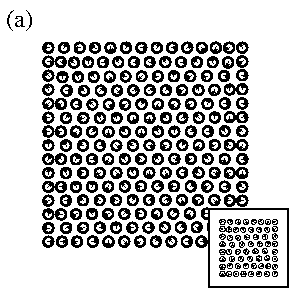
\includegraphics[height=0.27\textheight]{Nb198a_inset.pdf}
  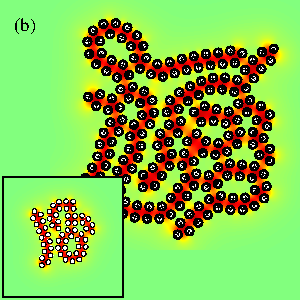
\includegraphics[height=0.27\textheight]{Nb198b_eta_inset.pdf}\\
  \hspace{1.55cm}
  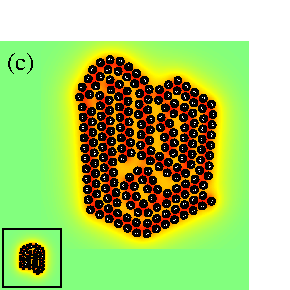
\includegraphics[height=0.27\textheight]{Nb198c_eta_inset.pdf}
  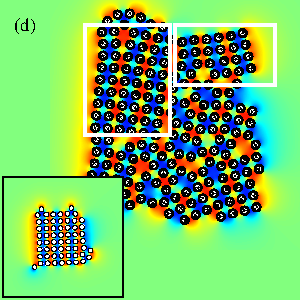
\includegraphics[height=0.27\textheight]{Nb198d_eta_inset.pdf}
\end{center}
\begin{caption}{\label{fig:relax}
  Panel (a) shows $N_b = 198$ particles confined to a square with random 
  positions and orientation.
  Depending on the boundary condition \eqref{eq:bc-type},
  the particles selc-assemble into distinct configurations.
  Panel (b) is for $b=1$ and the boundary condition mimicks that
  of an amphiphilic particle. 
  Panel (c) is for $b=2$ which gives rise to a multilamellar configuration. 
  In panel (d), the case $b = 0$ is for a water structure with
  positive/negative charge. 
  The false color maps use blue for $u < 0$, green for $u = 0$, and yellow then red for $u > 0$.}
\end{caption}
\end{figure}

\section{Equilibrium configurations}
\subsection{Boundary conditions and normalization}
The present paper considers boundary condition of the form
\begin{equation}
  \label{eq:bc-type}
g(\xx) = a(b + \cos \alpha),\quad a = (\pi c(2b^2 + 1))^{-1/2},\quad \xx \in \Gamma_i,
\end{equation}
where $\alpha$ is the angle between $\xx - \aa_i$ and the particle director
$\dd_i = (\cos \theta_i, \sin \theta_i)$.
The parameter $a$ normalizes the boundary conditions 
so that $\int_{\Gamma_i} g^2(\xx) \, \dif s = 1$.
We refer to the side of the particle where $\alpha = 0$
as the tail and the side where $\alpha = \pi$ as the head. 


To see the effect of the shift parameter $b$, we simulate the dynamics of
198 particles in a quiescent flow as shown in Figure~\ref{fig:relax}.
Three distinct configurations emerge:
(i) bilayers for $b = 1$, 
(ii) multilamellar for $b = 2$, and 
(iii) striated for $b = 0$.

Case (i) with $b = 1$, mimicks an amphiphilic particle.
The boundary condition $g$ is everywhere nonnegative,
takes the value $0$ on the
hydrophilic head,
and takes the maximum value $a$ on the
hydrophobic tail. 
The interaction is attractive, and particles collectively orient their
hydrophobic sides to form bilayers  (Figure~\ref{fig:relax}(b)). 

In case (ii) with $b = 1$, the boundary condition is positive everywhere.
It takes the maximum value $3a$ on tail and the
minimum value $a$ on the head side. 
Both sides of the Janus particle are hydrophobic but
moreso on the $\alpha = 0$ side.  
Over a short time scale, these particles also self-assemble into bilayers. But unlike for case (i),
the heads are also hydrophobic and so in the long-time dynamics
these bilayers also adhere to one another 
forming multilamella structures. Figure~\ref{fig:relax}(c), for example, shows a
multilamellar structure with 2 layers.
At equilibrium, the number of folds depends primarily on the number of particles.

A water structure with
positive/negative charge is possible in case (iii), $b = 0$
\cite{MaRa76, Ma77}.
Here, the head repels the tail of other particles
and the particles initially form chains with their directors perpendicular
to the length of the chain.  
The chains form stria
where the particles lie on a 
grid and the orientations alternate between layers (Figure~\ref{fig:relax}(d)).

The equilibrium configurations for case (ii) and (iii) are used as initial data in the
background flow simulations found in Section \ref{sec:results}.
In case (i), there are several connected
components forming isolated bilayers, micelles, and vesicles (Figure~\ref{fig:relax}(b)).
To have a single, coherent vesicle (i), we reinitialize
the case (i) particles in the form of a ring and run the relaxation procedure once more.


%\begin{figure}
%  \begin{center}
%  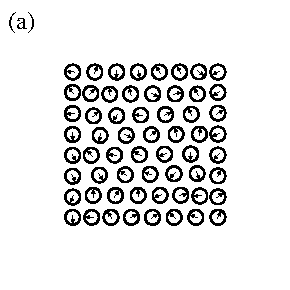
\includegraphics[height=0.15\textheight]{Nb60a.pdf}
%  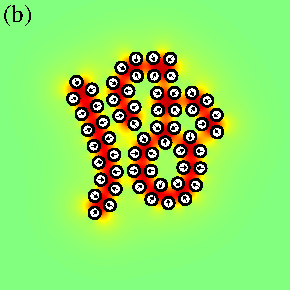
\includegraphics[height=0.15\textheight]{Nb60b.pdf}
%  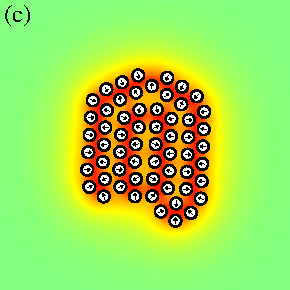
\includegraphics[height=0.15\textheight]{Nb60c.pdf}
% 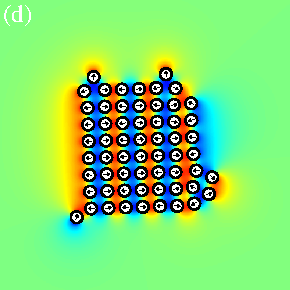
\includegraphics[height=0.15\textheight]{Nb60d.pdf}
%  \end{center}
%  \vspace{-20pt}  
%  \caption{\label{fig:relax_Nb60} 
%  }
%\end{figure}






\begin{figure}
  \begin{center}
%  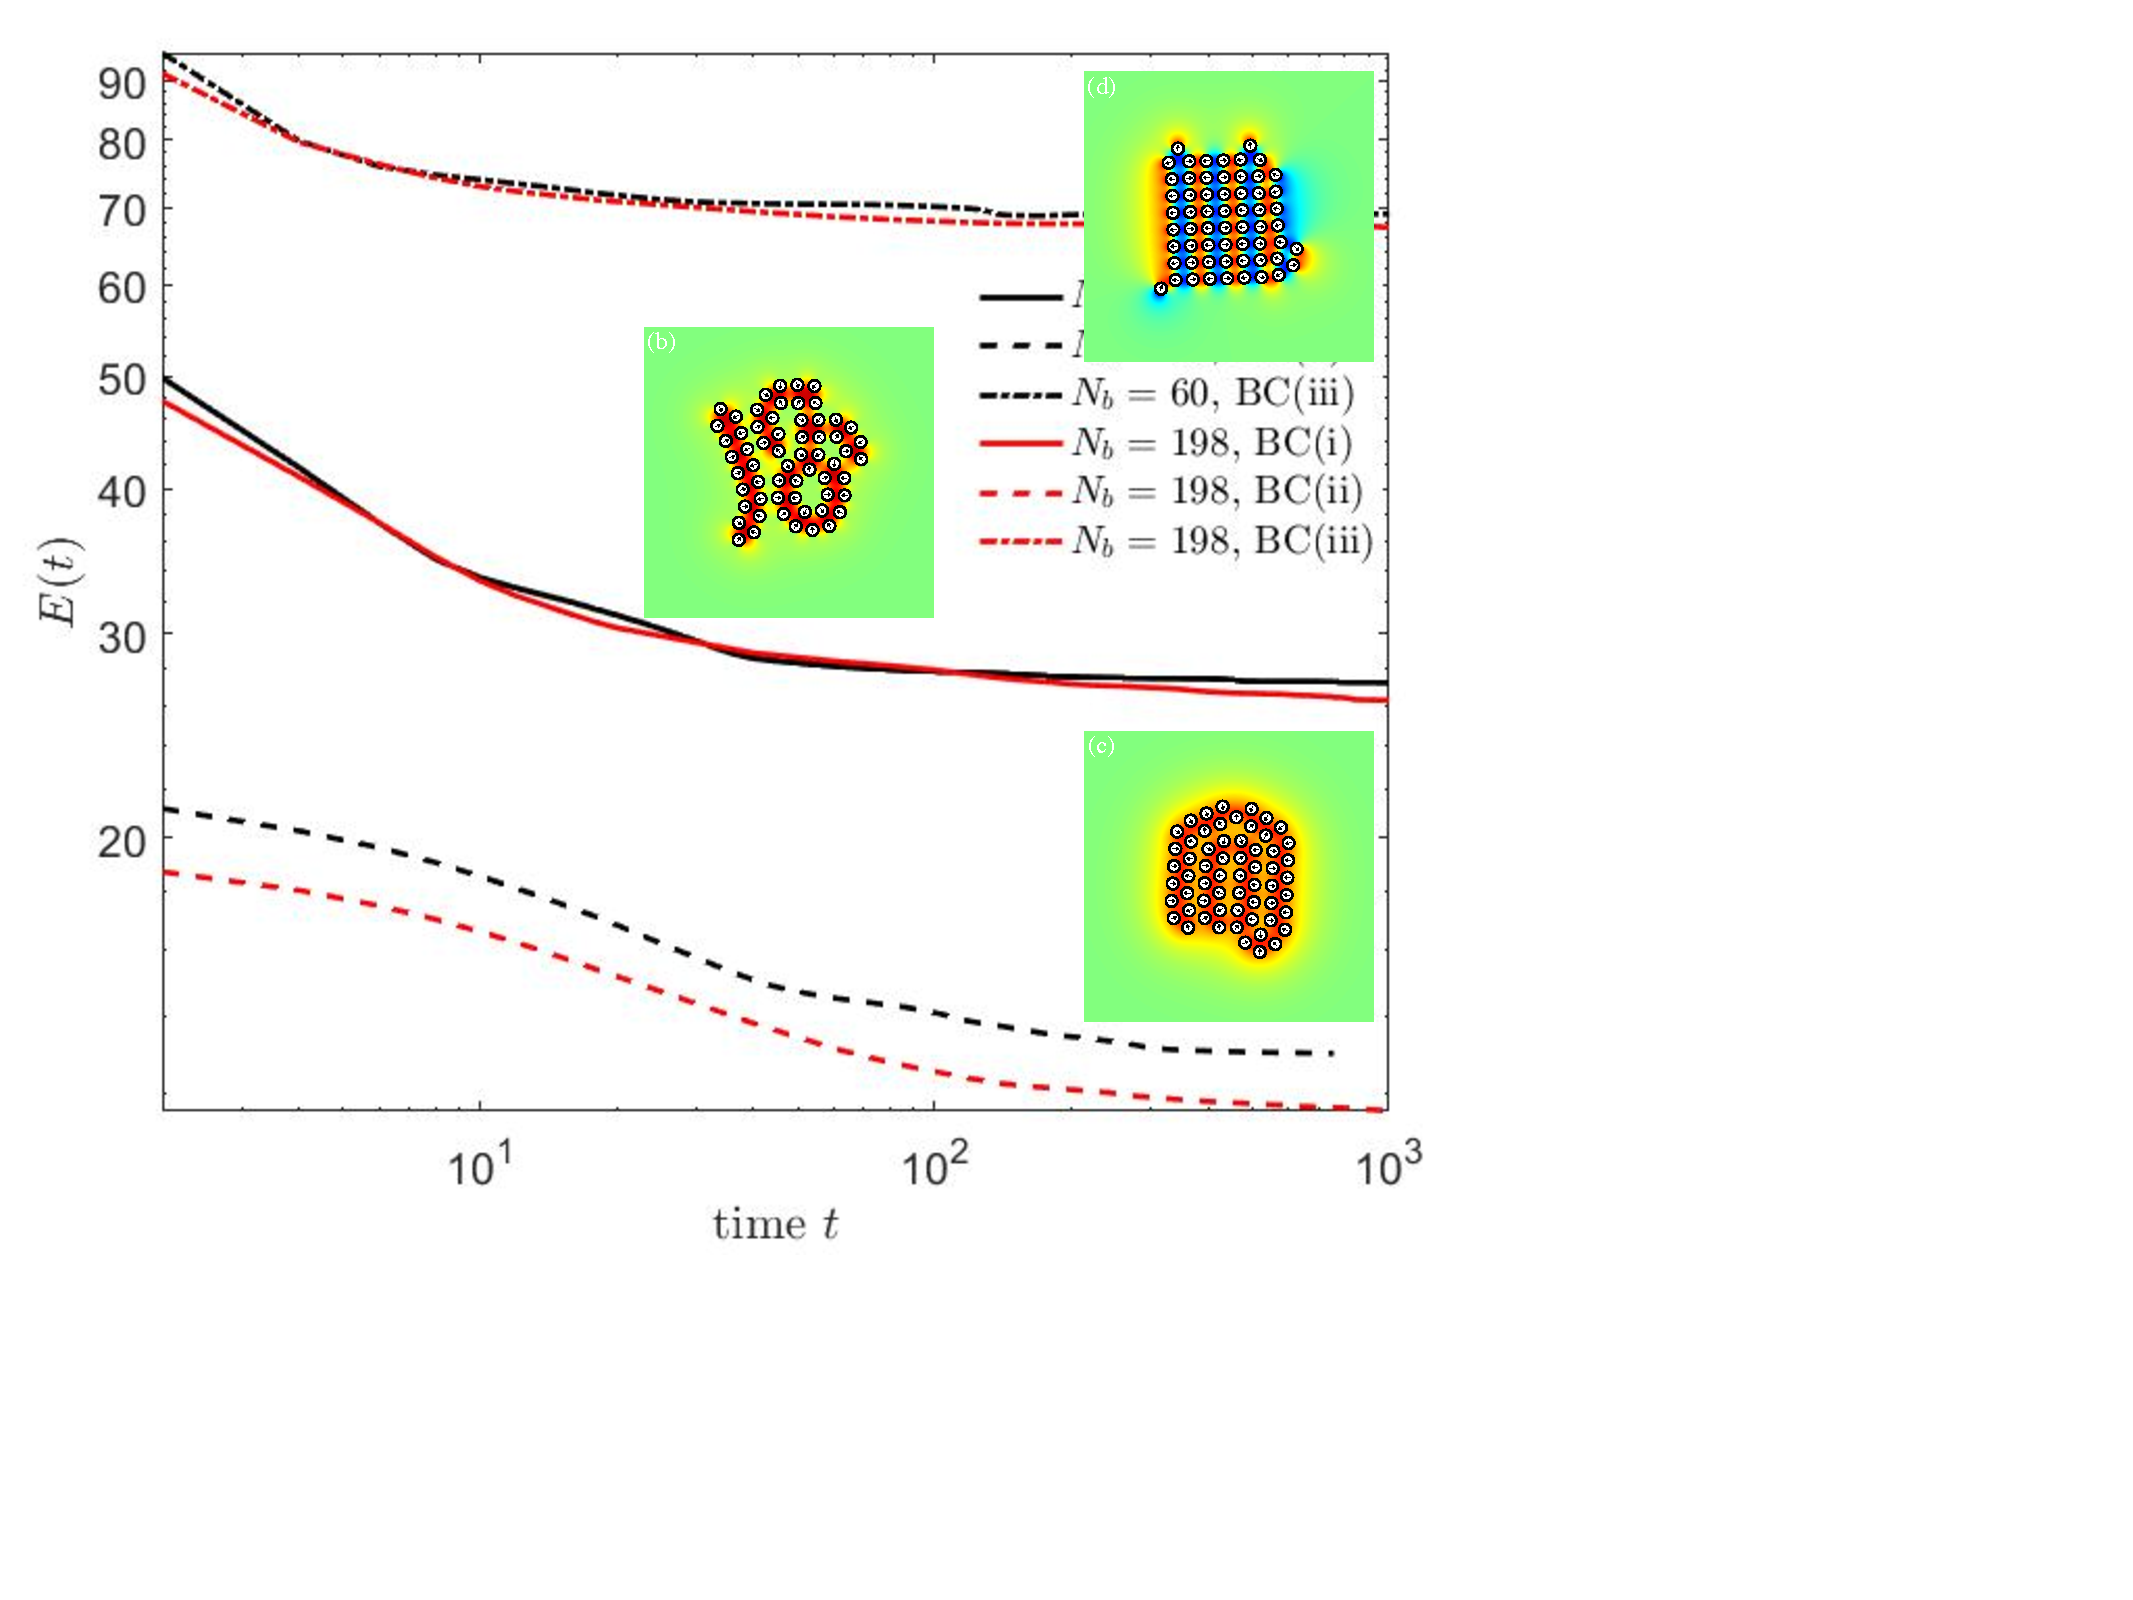
\includegraphics[width=0.49\textwidth]{Relax_Energy_inset.pdf}
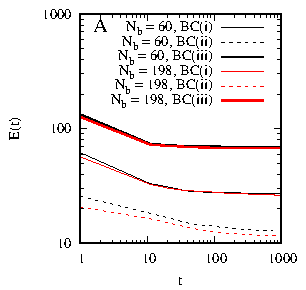
\includegraphics[width=0.49\textwidth]{relax_E.pdf}
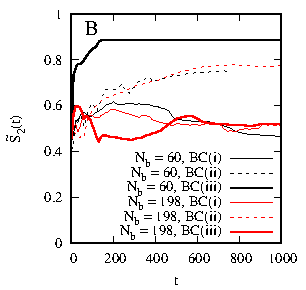
\includegraphics[width=0.49\textwidth]{relax_LOP.pdf} 
  \end{center}
  \vspace{-20pt}  
  \caption{\label{fig:relax_energy}
  A:  The free energy \eqref{eq:free_energy} is decreasing
    in the mobility problem formulation.  The initial energies
    are for the configuration in Figure \ref{fig:relax}a
    and the final energies are for the near-equilibrium
    configurations Figure \ref{fig:relax}b--c, respectively. 
    The red curves are the energies for the $N_b = 198$ cases normalized
    by $60/198$, showing that the energy approximately scales with the number of
    particles. B: The local order parameter $\tilde{S}_2$ for all 6 relaxation runs. The near-equilibrium configurations depend on the initial configuration and the results show that 
    the striated configurations have largest value of order parameter for both $N_b=60$ and $N_b=198$ cases.
  }
\end{figure}

\section{Measuring deformation}
We use the free energy $F$,
a Euclidean distance-based measure $d(t)$,
and a scalar order parameter $S_{2}(t)$ to measure
the deformation of particle configurations under background flows. 

First, we must simplify the
form of the free energy \eqref{eq:free_energy}
using integration by parts and \eqref{eq:SL}
to obtain
\begin{equation}
\label{eq:free_energy2}
F[u] = -\gamma
\int_{\Gamma} \rho g \nabla u \cdot \nnu \,\dif s
+ \frac{M}{2}
\sum_{j \neq i} 
P\left(\frac{|\aa_i - \aa_j|-2c}{\rho_0}\right).
\end{equation}
%
Here, we have substituted $g$ for $u$ since the boundary values are given.
However, evaluating $\nabla u \cdot \nnu$ on $\Gamma$ based on \eqref{eq:SL_BIE}
involves calculating a quadruple layer potential which has a
well-known obstacle in numerical implementation.
To overcome this obstacle, we use
%
\begin{equation}
\label{eq:normal_deriv}
\nabla u(\xx) \cdot \nnu(\xx)=
%\frac{\partial}{\partial \nnu_\xx} \DD[\sigma](\xx) =
-\frac{1}{\rho^2} {\bf t}_\xx\cdot \SSS[\sigma{\bf t}](\xx)
+ \frac{\dif}{\dif s}\SSS\left[\frac{\dif \sigma}{\dif s}\right](\xx), \quad \xx \in \Gamma.
\end{equation}
%
Here, ${\bf t}(\xx)$ is the tangent vector and $\dif/\dif s$ is the arclength derivative.
See the Appendix section \ref{sec:appendix} for the proof and details.
Substituting \eqref{eq:normal_deriv} into \eqref{eq:free_energy2} for the normal derivative
leads to single layer integral which is more straightforward to evaluate and we compute the
arclength derivative using spectrally accurate Fourier transform.
We have validated the form of \eqref{eq:normal_deriv} by extrapolating 
the primal energy \eqref{eq:free_energy} along test curves placed slightly
outside the particles. 

The Euclidian distance matrix is the $N_b \times N_b$ matrix 
$[D(t)]_{ij} = \|\aa_{i} - \aa_{j}\|$ for $i, j = 1, \dots, N_b$
To measure positional order, we use
\begin{equation}
\label{eq:EDM}
d(t) = \frac{1}{N_b^2}\|D(t) - D(0)\|
\end{equation}
where $\| \cdot \|$ is the Frobeneous norm.
For weak background flow strengths, the deformation in particle
configurations will be relatively small and the collection of
particles behaves as a rigid body i.e., $d(t) \ll 1$. 
 
To study orientational order, we use the scalar order parameter 
\begin{equation}
  \label{eq:S2}
S_2(t) = \frac{1}{N_b} \sum_{i=1}^{N_b} \frac{1}{2}(3\cos^2(\theta_i - \bar \theta) - 1).
\end{equation}
Here $\bar \theta$ is a circular mean defined as the
orientation of the largest eigenvalue eigenvector of 
$\dd_1\dd_1^\top + \dots + \dd_{N_b}\dd_{N_b}^\top$.
A value $S_2(t) = 1$ indicates a complete orientational
order where all particle directors lie on a common axis e.g.,
two parallel vectors with possibly opposite direction are ordered. 
A value far from 1 indicates disorder.

The measure $S_2$ is an inadequate for the bilayer and
multilamellar structures.  For example, the directors of a circular
bilayer vesicle are uniformly distributed along a circle, even though
there is a strong orientational order between neighboring particles.
To account for these latter cases, we use
\begin{equation}
  \label{eq:localS2}
\tilde{S}_2(t) = \frac{1}{N_b} \sum_{i=1}^{N_b}
\frac{1}{2}(3\cos^2(\theta_i - \bar \theta_i) - 1).
\end{equation}
where $\bar \theta_i$ is the circular mean restricted to particles
indexed by $j$ for which $\|\aa_i - \aa_j\| < 4c$. In practice, if a particle is
isolated and has no neighbors within a distance $4c$, then we exclude it from
the sum \eqref{eq:localS2}. 

\section{Results}
\label{sec:results}


%\begin{figure}
%\caption{\label{fig:ves_shear} A vesicle in shear flow}
%\end{figure}
%\begin{figure}
%\caption{\label{fig:ves_shear} A vesicle in Taylor-Green flow}
%\end{figure}
\begin{figure}
  \begin{center}
  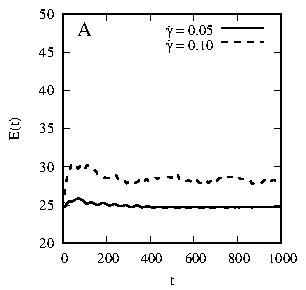
\includegraphics[width=0.3\textwidth]{VS_E.pdf}
   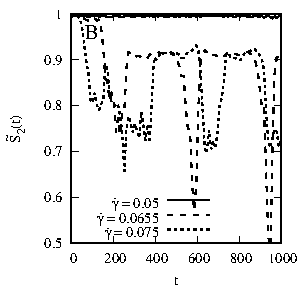
\includegraphics[width=0.3\textwidth]{VS_LOP.pdf}
    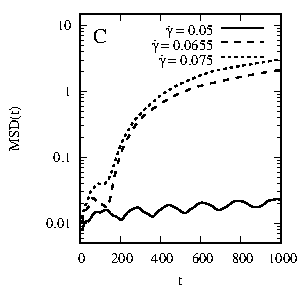
\includegraphics[width=0.3\textwidth]{VS_MSD.pdf}\\
      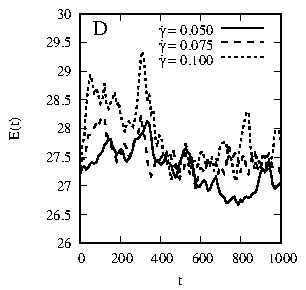
\includegraphics[width=0.3\textwidth]{BS_E.pdf}
   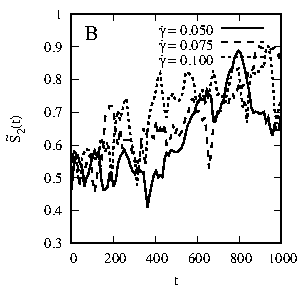
\includegraphics[width=0.3\textwidth]{BS_LOP.pdf}
    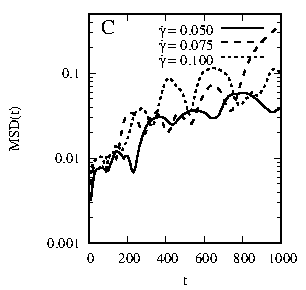
\includegraphics[width=0.3\textwidth]{BS_MSD.pdf}
  \end{center}
  \caption{
    \label{fig:BC1_shear}
    The quantities $E(t)$, $\tilde S_2(t)$, and $d(t)$
    are indicators of bilayer (case (i)) deformation at various shear rates. }
\end{figure}


\begin{figure}
  \begin{center}
      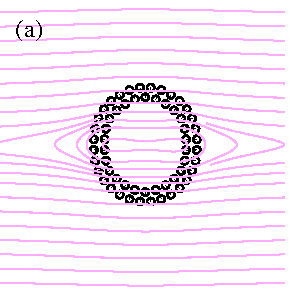
\includegraphics[width=0.22\textwidth]{VS_0.pdf}
      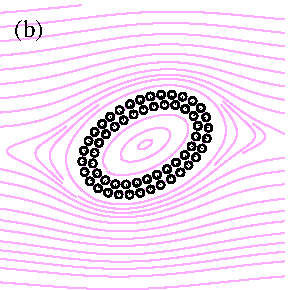
\includegraphics[width=0.22\textwidth]{VS_1.pdf}
   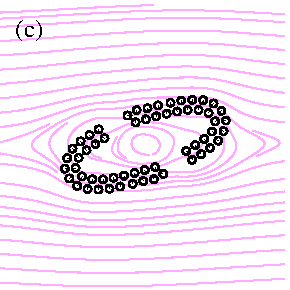
\includegraphics[width=0.22\textwidth]{VS_2.pdf}
   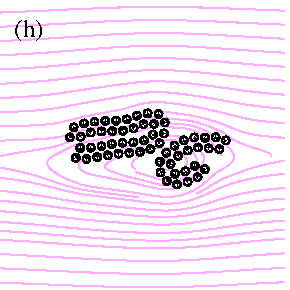
\includegraphics[width=0.22\textwidth]{VS_3.pdf}\\
         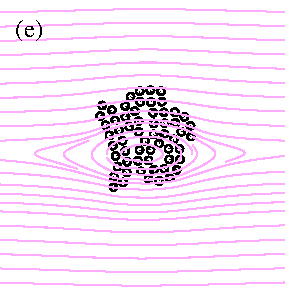
\includegraphics[width=0.22\textwidth]{BS_0.pdf}
      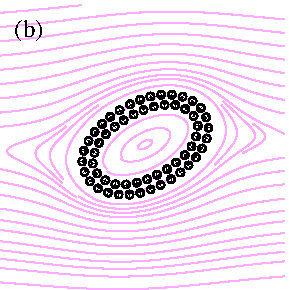
\includegraphics[width=0.22\textwidth]{BS_1.pdf}
   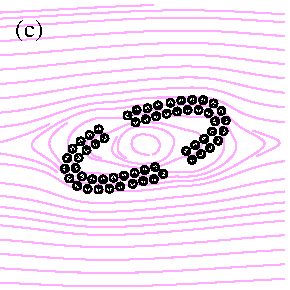
\includegraphics[width=0.22\textwidth]{BS_2.pdf}
   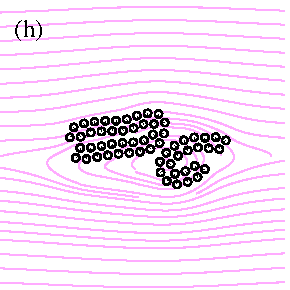
\includegraphics[width=0.22\textwidth]{BS_3.pdf}
%   Panels (e)-(f) same but for non-vesicle initial configuration
  \end{center}
  \caption{
    \label{fig:BC1_shear_flow}
    The figure shows a vesicle in shear flow (panels (a)-(d), $\dot \gamma = ...$) 
    and the multiple component bilayers in shear (panels (e)-(f), $\dot \gamma = ...$).}
\end{figure}

\subsection{Boundary condition (i):   bilayer configurations}
The vesicle in a shear flow undergoes the familiar tank-treading deformation.
Our previous paper \cite{Fu2022_JFM} studied the geometry,
intermonolayer slip, and critical shear rates $\gamma^*$
for vesicles comprised of amphiphilic Janus particles. 

The vesicle is subject to a shear background flow
\begin{equation}
\uu_\infty(\xx) = \dot\gamma ({\bf e}_y\cdot\xx){\bf e}_x,
\end{equation}
%
where $\dot\gamma$ is the shear rate. Figure~\ref{fig:shear_1} (a)--(c)
shows snapshots of the vesicle when $\dot\gamma= ... $ is
below the critical shear rate $\dot \gamma_* = ...$
Here, the free energy and order parameter are more or less constant
(Figure \ref{fig:BC1_shear}ab, solid curves).  The is a slight upward shift
in $d(t)$ (Figure \ref{fig:BC1_shear}c, solid curve) due to relative
displacement as the two leaflets slide past one another.  

%\begin{figure}
%\caption{\label{fig:ves_shear} A vesicle in shear flow}
%\end{figure}
%\begin{figure}
%\caption{\label{fig:ves_shear} A vesicle in Taylor-Green flow}
%\end{figure}




In, Figure~\ref{fig:shear_2} (a)--(c), 
$\dot\gamma= ...$ is above the critical shear rate,
and there is a jump in energy (Figure \ref{fig:BC1_shear}a, dashed curve)
due to the breaking of the vesicle into two components.  
There is greater variation in the order parameter $\tilde{S}_2(t)$ as well
with a baseline value around $0.7$
(Figure \ref{fig:BC1_shear}b, dashed curve).The oscillations occur due to the
orbit of the two bilayer components, and $\tilde{S}_2(t)$ increases
to about $0.9$ when the components are nearly parallel and slide past one another.
Positional order, however, diverges since the two component configuration
is uncorrelated to the initial circular configuration (Figure \ref{fig:BC1_shear}c, dashed curve).






%

The Taylor-Green (TG) background flow is
\begin{equation}
  \uu_\infty(\xx) = V_0 \left(-\cos({\bf e}_x\cdot\xx/l)\sin({\bf e}_y\cdot\xx/l){\bf e}_x
  +\sin({\bf e}_x\cdot\xx/l)\cos({\bf e}_y\cdot\xx/l){\bf e}_y\right).
\end{equation}
where $l$ sets the size of the rotating cells and $V_0$ is the flow strength. 
%


\begin{figure}
  \begin{center}
  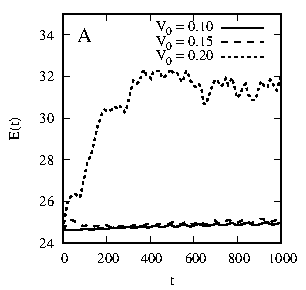
\includegraphics[width=0.3\textwidth]{VTG_E.pdf}
   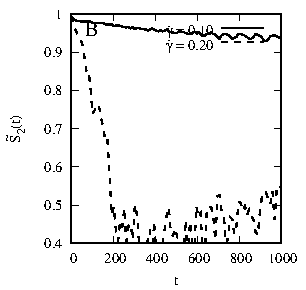
\includegraphics[width=0.3\textwidth]{VTG_LOP.pdf}
    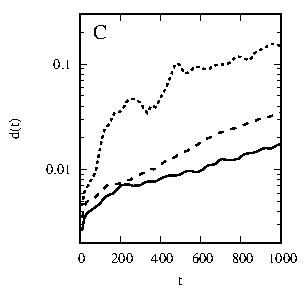
\includegraphics[width=0.3\textwidth]{VTG_MSD.pdf}\\
  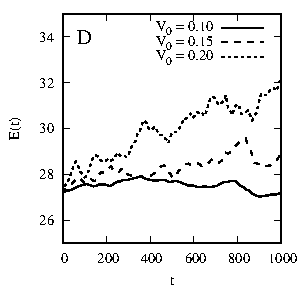
\includegraphics[width=0.3\textwidth]{BTG_E.pdf}
   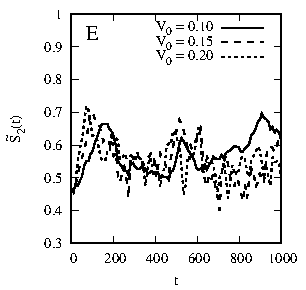
\includegraphics[width=0.3\textwidth]{BTG_LOP.pdf}
    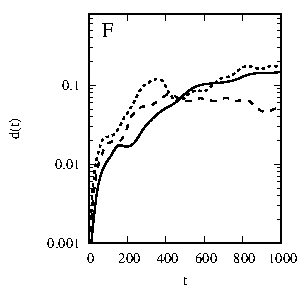
\includegraphics[width=0.3\textwidth]{BTG_MSD.pdf}
  \end{center}
\caption{A vesicle in Taylor-Green flows when the flow strength $V_0=\{0.1, 0.15, 0.2\}$. }
\end{figure}


\begin{figure}
  \begin{center}
  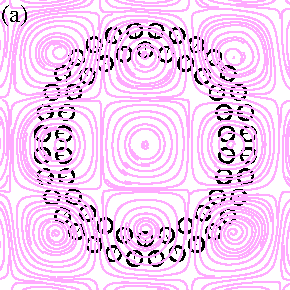
\includegraphics[width=0.22\textwidth]{VTG_0.pdf}
  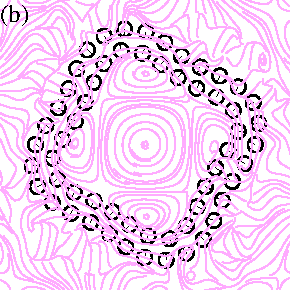
\includegraphics[width=0.22\textwidth]{VTG_1.pdf}
  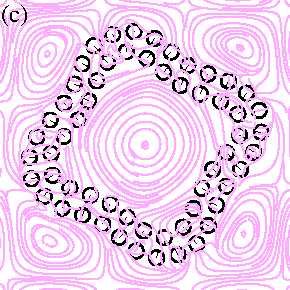
\includegraphics[width=0.22\textwidth]{VTG_2.pdf} 
    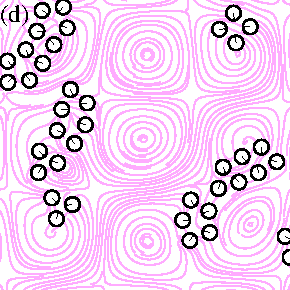
\includegraphics[width=0.22\textwidth]{VTG_3.pdf} \\
      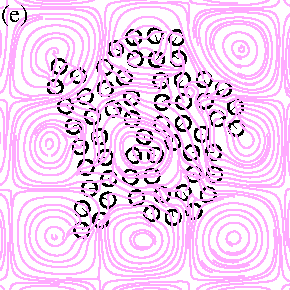
\includegraphics[width=0.22\textwidth]{BTG_0.pdf}
  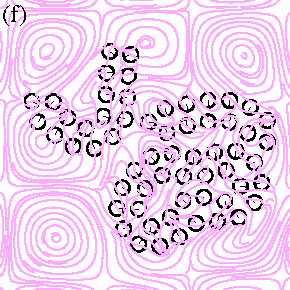
\includegraphics[width=0.22\textwidth]{BTG_1.pdf}
  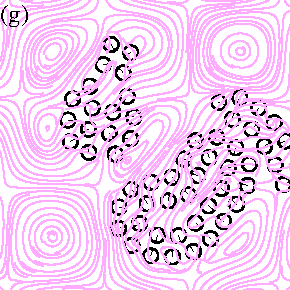
\includegraphics[width=0.22\textwidth]{BTG_2.pdf} 
    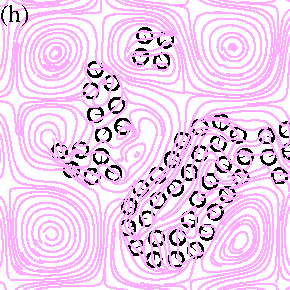
\includegraphics[width=0.22\textwidth]{BTG_3.pdf}
  \end{center}
  \vspace{-20pt}  
  \caption{\label{fig:BTG_flow} Snapshots of simulation using boundary condition \eqref{eq:bcs}(ii) in a shear flow when $\dot\gamma=0.05$. }
\end{figure}

\begin{figure}
  \begin{center}
  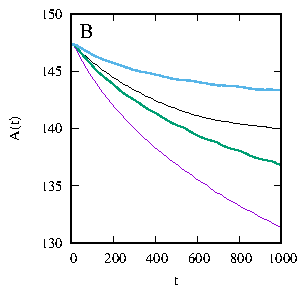
\includegraphics[width=0.4\textwidth]{VTG_Area}
  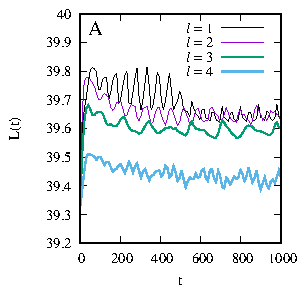
\includegraphics[width=0.4\textwidth]{VTG_Len}
  \end{center}
  \vspace{-20pt}  
  \caption{\label{fig:VTG_AreaLen} Snapshots of simulation using boundary condition \eqref{eq:bcs}(ii) in a shear flow when $\dot\gamma=0.05$. }
\end{figure}

\begin{figure}
  \begin{center}
  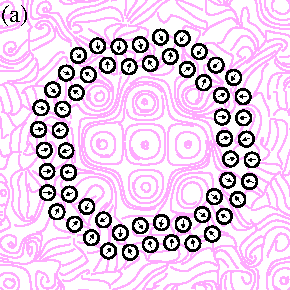
\includegraphics[width=0.22\textwidth]{VTG_Scale_0.pdf}
  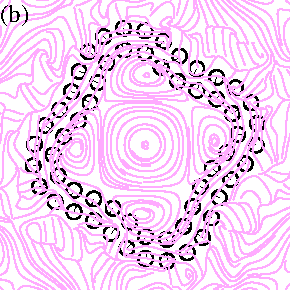
\includegraphics[width=0.22\textwidth]{VTG_Scale_1.pdf}
  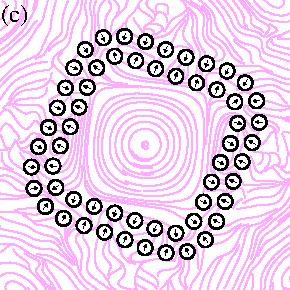
\includegraphics[width=0.22\textwidth]{VTG_Scale_2.pdf} 
    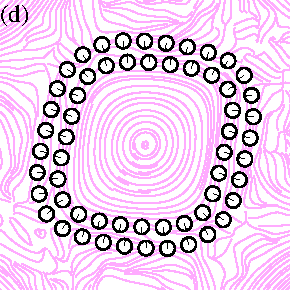
\includegraphics[width=0.22\textwidth]{VTG_Scale_3.pdf}
      \end{center}
  \vspace{-20pt}  
  \caption{\label{fig:BTG_Scale_flow} Snapshots of simulation using boundary condition \eqref{eq:bcs}(ii) in a shear flow when $\dot\gamma=0.05$. }
\end{figure}

%
%\begin{figure}
%  \begin{center}
%  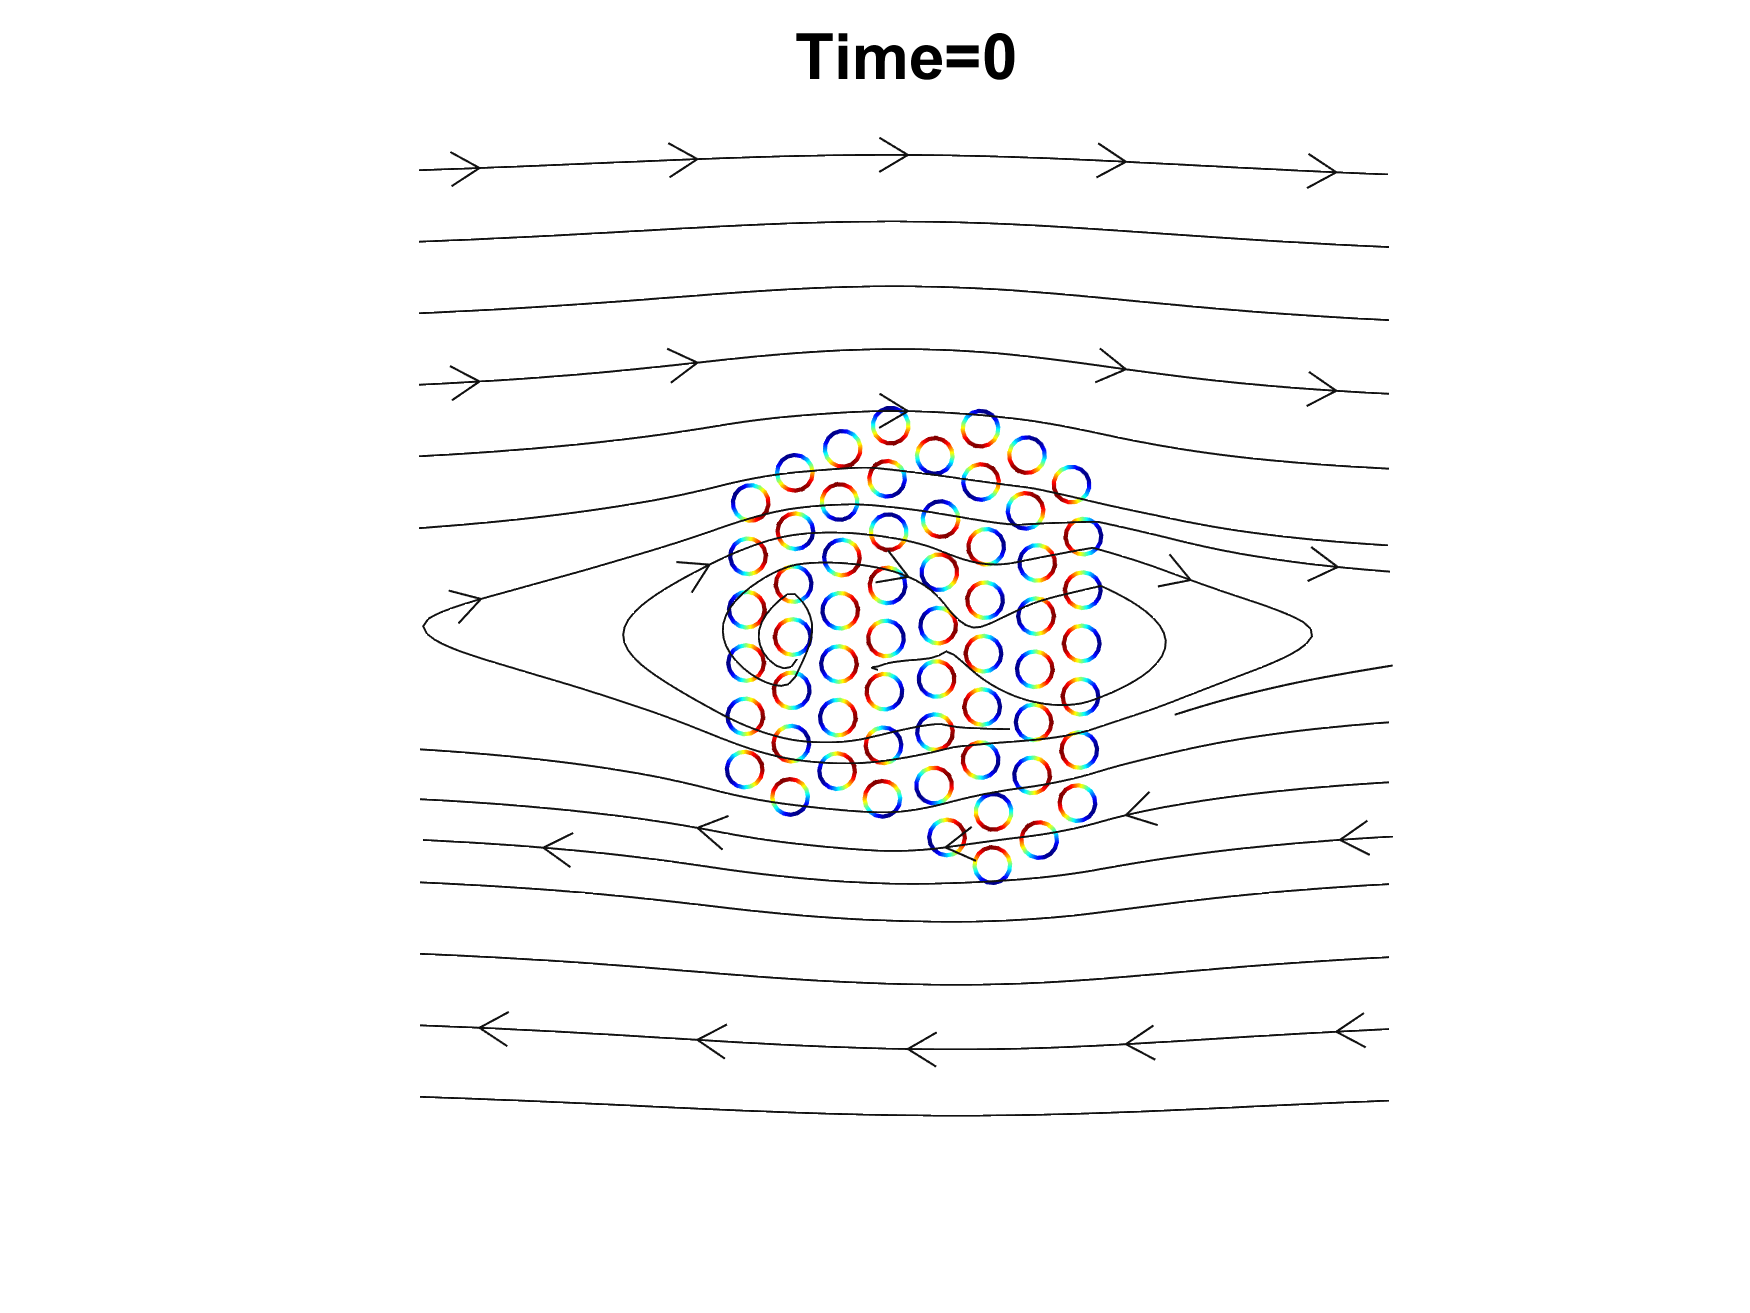
\includegraphics[width=0.32\textwidth]{shear_0.png}
%  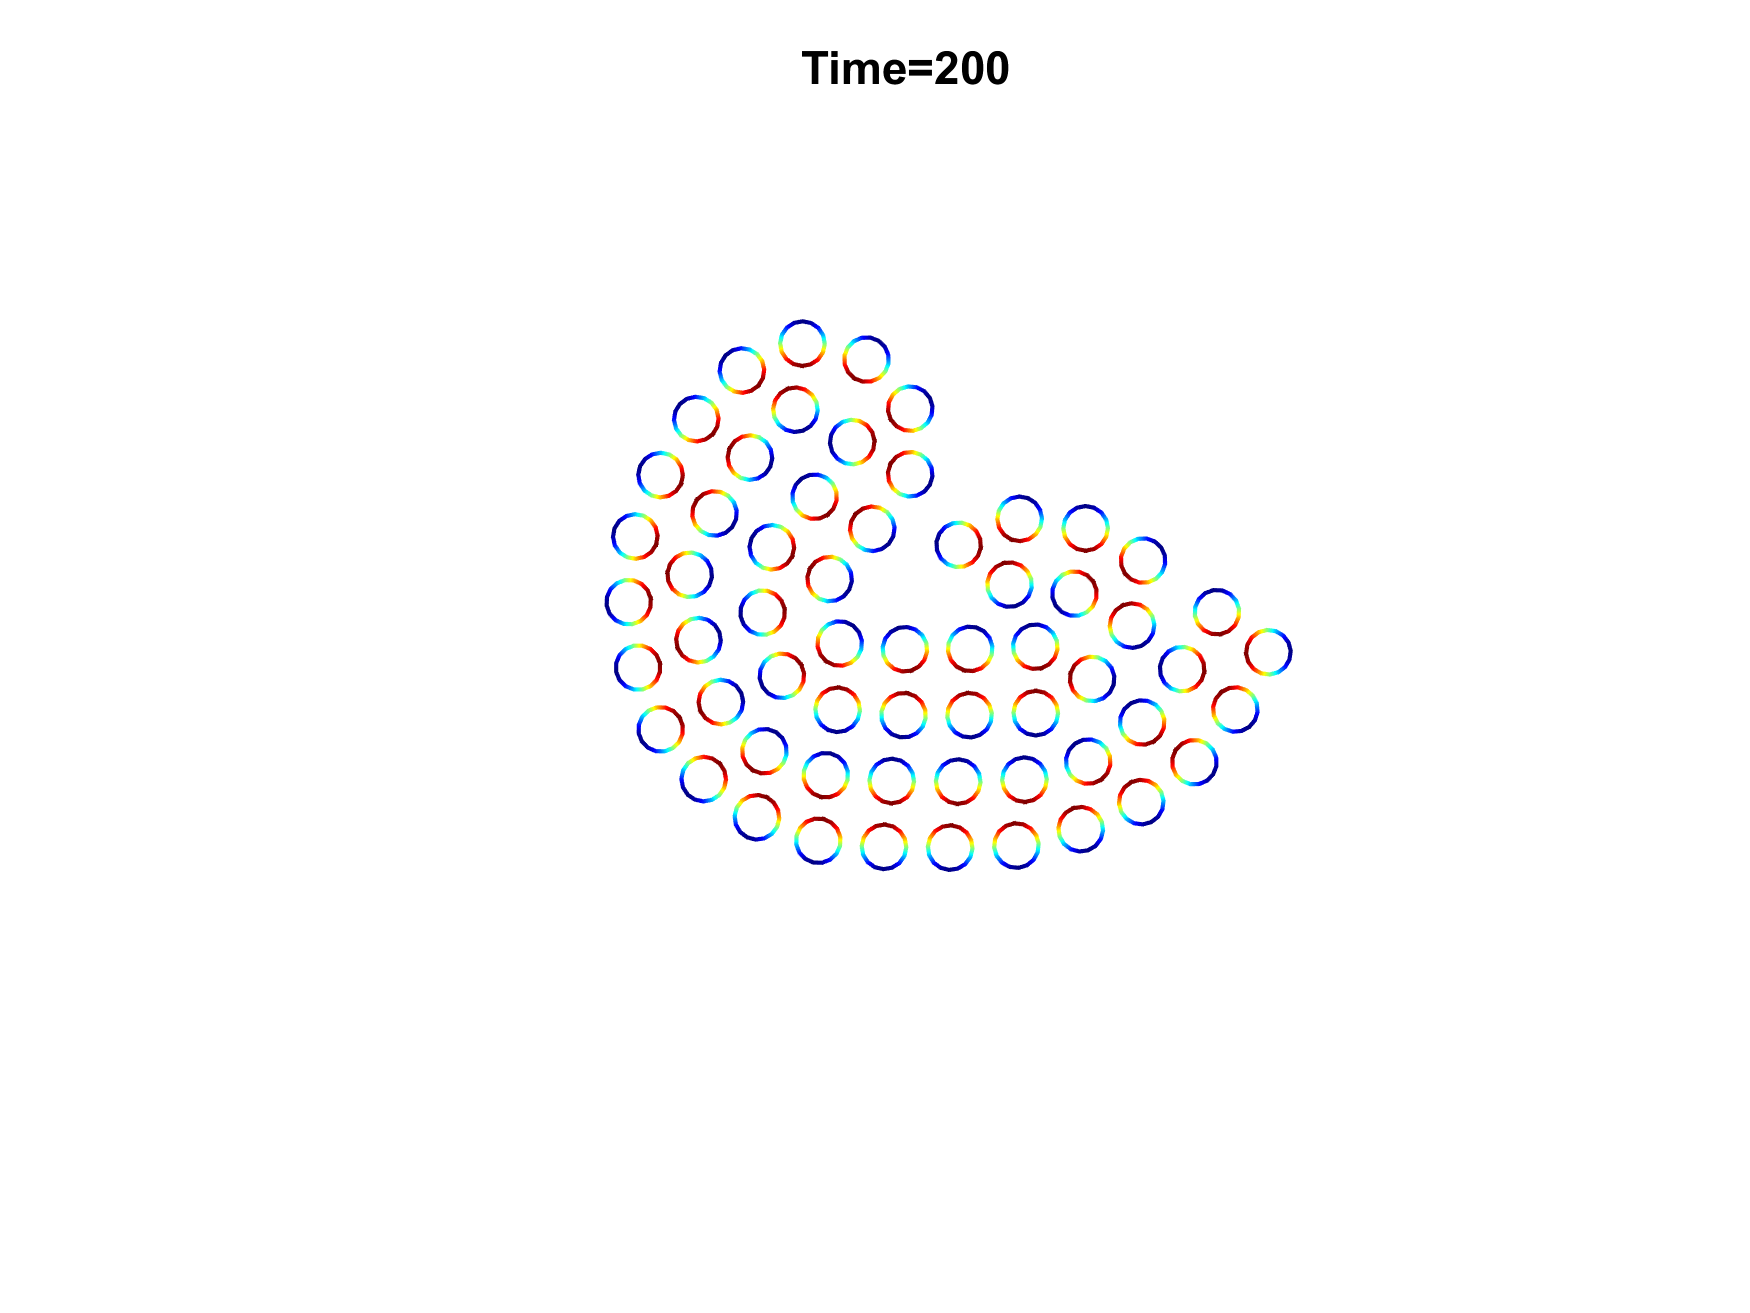
\includegraphics[width=0.32\textwidth]{shear_1000.png}
%  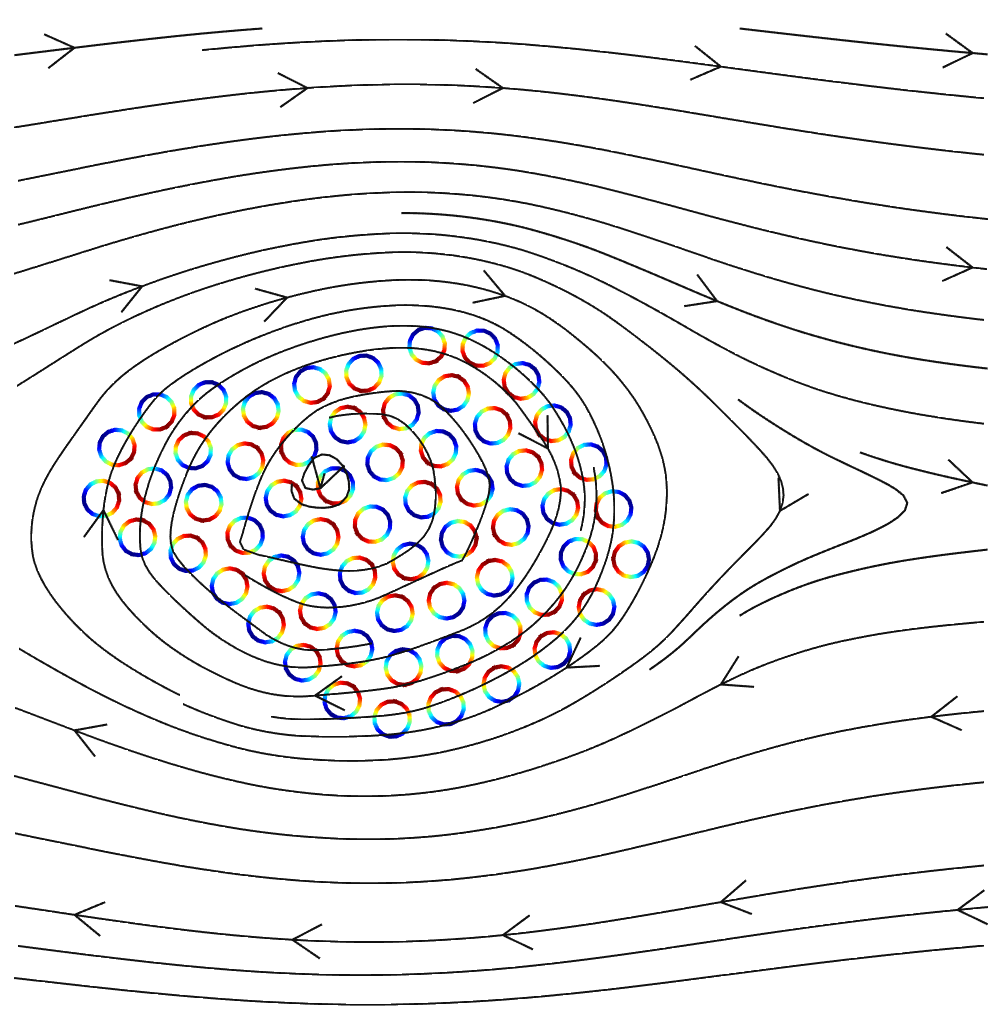
\includegraphics[width=0.32\textwidth]{shear_2000.png} 
%  \end{center}
%  \vspace{-20pt}  
%  \caption{\label{fig:shear_1} Snapshots of simulation using boundary condition \eqref{eq:bcs}(ii) in a shear flow when $\dot\gamma=0.05$. }
%\end{figure}
%
%\begin{figure}
%  \begin{center}
%  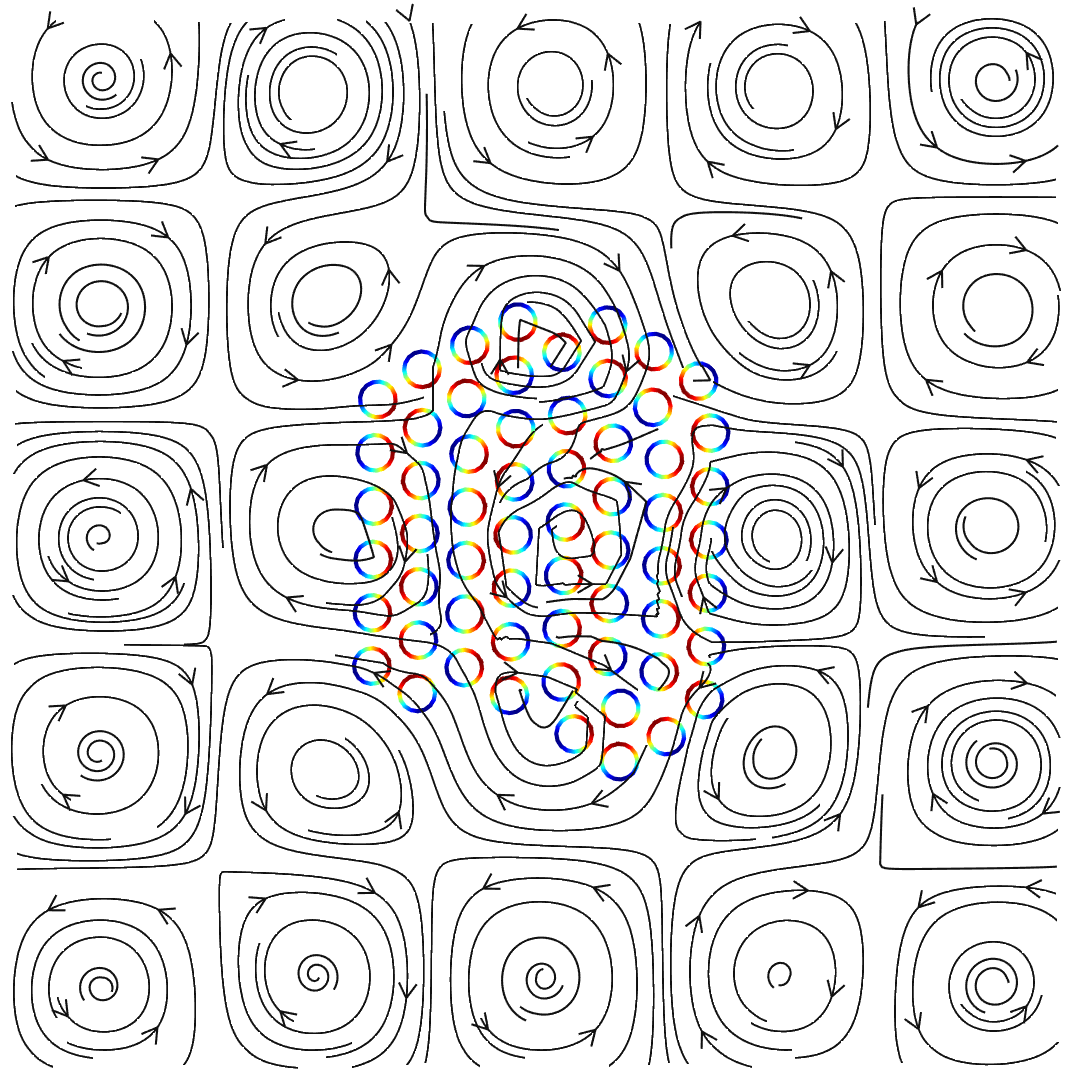
\includegraphics[width=0.32\textwidth]{TG_0.png}
%  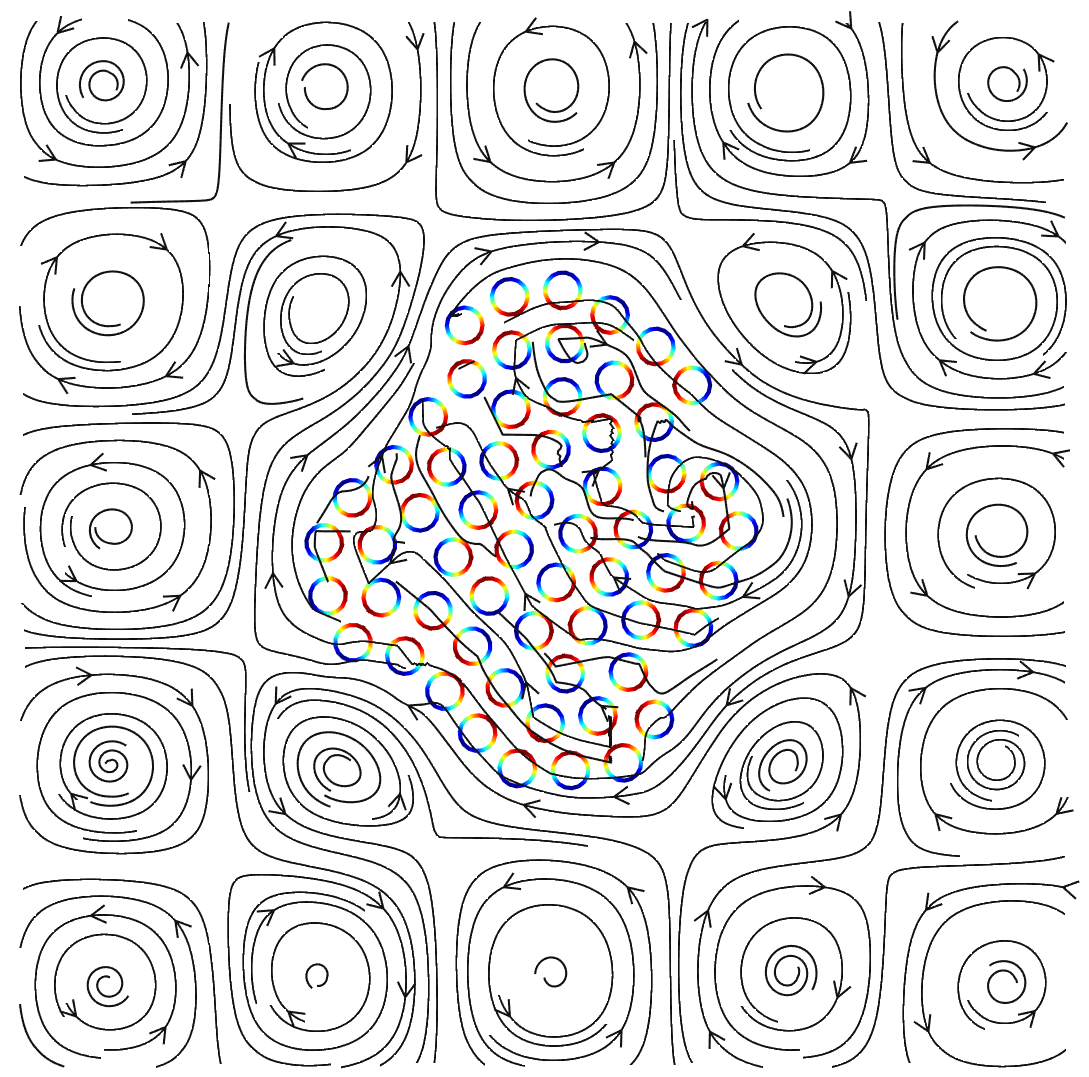
\includegraphics[width=0.32\textwidth]{TG_2500.png}
%  \includegraphics[width=0.32\textwidth]{TG_5000.png}
%  \end{center}
%  \vspace{-20pt}  
%  \caption{\label{fig:TG_1} Snapshots of simulation using boundary condition \eqref{eq:bcs}(b) in a Taylor-Green flow when $V_0=0.1$ and $l=0.5$.}
%\end{figure}
\subsection{Boundary condition (ii):  multilamellar configurations}

\begin{figure}
  \begin{center}
  \includegraphics[width=0.3\textwidth]{MS_E.pdf}
   \includegraphics[width=0.3\textwidth]{MS_LOP.pdf}
    \includegraphics[width=0.3\textwidth]{MS_MSD.pdf}
  \end{center}
      \caption{A multi-lamellar structure in shear flows with shear rates $\dot\gamma=\{0.05, 0.1, 0.15\}$. We compute the energy and the mean square displacement $MSD(t) = \frac{1}{N_b^2}\sum_{i=1}^{N_b} ||D(t)-D(0) ||_2$ where the matrix $D$ is the pairwise distance matrix at time $t$.    }
\end{figure}


\begin{figure}
  \begin{center}
  \includegraphics[width=0.22\textwidth]{MS_0.pdf}
  \includegraphics[width=0.22\textwidth]{MS_1.pdf}
  \includegraphics[width=0.22\textwidth]{MS_2.pdf} 
    \includegraphics[width=0.22\textwidth]{MS_3.pdf} 
  \end{center}
  \vspace{-20pt}  
  \caption{\label{fig:MS_flow} Snapshots of simulation using boundary condition \eqref{eq:bcs}(ii) in a shear flow when $\dot\gamma=0.05$. }
\end{figure}






\begin{figure}
  \begin{center}
  \includegraphics[width=0.3\textwidth]{MTG_E.pdf}
   \includegraphics[width=0.3\textwidth]{MTG_LOP.pdf}
    \includegraphics[width=0.3\textwidth]{MTG_MSD.pdf}
  \end{center}
    \caption{A multi-lamellar structure in a Taylor-Green flow when the flow strength $V_0=\{0.1,0.15,0.2\}$. }
\end{figure}

\begin{figure}
  \begin{center}
  \includegraphics[width=0.22\textwidth]{MTG_0.pdf}
  \includegraphics[width=0.22\textwidth]{MTG_1.pdf}
  \includegraphics[width=0.22\textwidth]{MTG_2.pdf} 
    \includegraphics[width=0.22\textwidth]{MTG_3.pdf} 
  \end{center}
  \vspace{-20pt}  
  \caption{\label{fig:MTG_flow} Snapshots of simulation using boundary condition \eqref{eq:bcs}(ii) in a shear flow when $\dot\gamma=0.05$. }
\end{figure}


%\begin{figure}
%  \begin{center}
%  \includegraphics[width=0.21\textwidth]{shear_checker_0.png}
%  \includegraphics[width=0.21\textwidth]{shear_checker_250.png}
%  \includegraphics[width=0.21\textwidth]{shear_checker_500.png}
%  \includegraphics[width=0.21\textwidth]{shear_checker_750.png} \\
%%  \includegraphics[width=0.4\textwidth]{lambda_fig1.jpg}
%  \end{center}
%  \vspace{-20pt}  
%  \caption{\label{fig:shear_1} Snapshots of simulation using boundary condition \eqref{eq:bcs}(ii) in a shear flow when $\dot\gamma=0.05$. }
%\end{figure}
%
\subsection{Boundary condition (iii): striated configurations} 

\begin{figure}
  \begin{center}
  \includegraphics[width=0.3\textwidth]{CS_E.pdf}
   \includegraphics[width=0.3\textwidth]{CS_LOP.pdf}
    \includegraphics[width=0.3\textwidth]{CS_MSD.pdf}
  \end{center}
\caption{A checker board in shear flows with shear rates $\dot\gamma=\{0.125, 0.15\}$. We propose the order parameter defined by $S_{loc} = \frac12(3\cos(\theta-\bar\theta)^2-1)$}
\end{figure}


\begin{figure}
  \begin{center}
  \includegraphics[width=0.22\textwidth]{CS_0.pdf}
  \includegraphics[width=0.22\textwidth]{CS_1.pdf}
  \includegraphics[width=0.22\textwidth]{CS_2.pdf} 
    \includegraphics[width=0.22\textwidth]{CS_3.pdf} 
  \end{center}
  \vspace{-20pt}  
  \caption{\label{fig:CS_flow} Snapshots of simulation using boundary condition \eqref{eq:bcs}(ii) in a shear flow when $\dot\gamma=0.05$. }
\end{figure}


\begin{figure}
  \begin{center}
  \includegraphics[width=0.3\textwidth]{CTG_E.pdf}
   \includegraphics[width=0.3\textwidth]{CTG_LOP.pdf}
    \includegraphics[width=0.3\textwidth]{CTG_MSD.pdf}
  \end{center}
\caption{A checker board in Taylor-Green flows when the flow strength $V_0=\{0.2,0.3\}$. }
\end{figure}

\begin{figure}
  \begin{center}
  \includegraphics[width=0.22\textwidth]{CTG_0.pdf}
  \includegraphics[width=0.22\textwidth]{CTG_1.pdf}
  \includegraphics[width=0.22\textwidth]{CTG_2.pdf} 
    \includegraphics[width=0.22\textwidth]{CTG_3.pdf} 
  \end{center}
  \vspace{-20pt}  
  \caption{\label{fig:CTG_flow} Snapshots of simulation using boundary condition \eqref{eq:bcs}(ii) in a shear flow when $\dot\gamma=0.05$. }
\end{figure}

\section{Discussion}
\begin{figure}
  \begin{center}
  \includegraphics[height=0.2\textheight]{multilamellar_shear0p1_Energy_LsFs}
    \includegraphics[height=0.2\textheight]{multilamellar_shear0p1_MSD_LsFs}
  \end{center}
    \caption{ A multi-lamellar structure in a shear flow when the shear rate is $\dot\gamma=0.1$. We tune the length scale parameters, radius, $\rho$ and $\rho_0$, by $\pm 5\%$ and the force scale parameters, $\gamma$ and $M$, by $\pm 5\%$.    }
\end{figure}

It is worth noting that in the dipolar molecules modeled by
Laplace equation, the equilibrium configurations consist of strands,
rather than a patch, of particles and also have
alternating orientations \cite{}. 


\section{Appendix}
\label{sec:appendix}
To prove \eqref{eq:normal_deriv}, let 
\begin{equation}
  \label{eq:SLP}
  \mathcal{S}[\sigma](\xx) = \int_\Gamma G(\xx-\yy) \sigma(\yy)\, \dif s_\yy
\end{equation}
be the single layer potential for a density function $\sigma.$
Fix $\xx \in \Gamma$,
let $\nnu_{\xx} = \nnu(\xx)$ and $\nnu_{\yy}$ be the unit normal at $\xx$, respectively $\yy$, in $\Gamma$,
and let $\zz \in \Omega$.  The subscripts in $\nabla_{\zz}$ and $\nabla_{\yy}$ denote
differentiation with respect to $\zz$, respectively $\yy$.

Recall from \eqref{eq:SL_BIE} that $u = \mathcal{D}[\sigma]$.
Then  
\begin{align*}
\nabla_{\zz} u(\zz) \cdot \nnu_{\xx}
&=\nnu_\xx \cdot \nabla_\zz \int_\Gamma \frac{\partial G(\zz-\yy)}{\partial \nnu_\yy}\sigma(\yy) \,\dif s_\yy\\
&=\int_\Gamma \nnu_\xx^\top \left(\nabla_\zz\nabla_\yy^\top  G(\zz-\yy)\right) \nnu_\yy\sigma(\yy)  \,\dif s_\yy\\
  &=-\int_\Gamma \nnu_\xx^\top \left(\nabla_\yy\nabla_\yy^\top G(\zz-\yy)\right)\nnu_\yy\sigma(\yy)\ \dif s_\yy,
\end{align*}
since we can interchange $\nabla_\zz$ with $-\nabla_\yy$.
Following \cite{Hsiao2008}, \S 1.2,
\[
\nnu_\xx^\top \left(\nabla_\yy\nabla_\yy^\top G(\zz-\yy)\right)\nnu_\yy
=
-\tt_{\xx}^\top \left(\nabla_\yy\nabla_\yy^\top G(\zz-\yy)\right)\tt_{\yy}
+ \Delta_{\yy}G(\zz-\yy) \tt_{\xx}\cdot \tt_{\yy}
\]
Then, using that $\Delta_{\yy} G(\zz-\yy) = \rho^{-2} G(\zz-\yy)$,
interchanging $\nabla_\yy$ with $-\nabla_\zz$ once more,
and integrating by parts in arclength $s$,
we obtain 
\begin{align*}
\nabla_{\zz} u(\zz) \cdot \nnu_{\xx}
&=-\int_\Gamma  \Delta_\yy G(\zz-\yy) {\bf t}_\xx \cdot   {\bf t}_\yy \sigma(\yy)\ \dif s_\yy
+\int_\Gamma({\bf t}_\xx\cdot\nabla_\yy)({\bf t}_\yy\cdot\nabla_\yy G(\zz-\yy))\sigma(\yy)\ \dif s_\yy\\
&= -\int_\Gamma \frac{1}{\rho^{2}} G(\zz-\yy) {\bf t}_\xx \cdot {\bf t}_\yy \sigma(\yy)\ \dif s_\yy  
-({\bf t}_\xx\cdot\nabla_\zz)\int_\Gamma \frac{\dif}{\dif s_\yy}G(\zz-\yy) \sigma(\yy)\ \dif s_\yy\\
&= -\frac{1}{\rho^2} {\bf t}_\xx\cdot \int_\Gamma G(\zz-\yy){\bf t}_\yy \sigma(\yy)\ \dif s_\yy + 
({\bf t}_\xx \cdot \nabla_\zz)\int_\Gamma G(\zz-\yy)\frac{\dif }{\dif s} \sigma(\yy)  \dif s_\yy.
\end{align*}
%
Letting $\zz\to\xx\in\Gamma$, and noting that both sides of the equation are continuous,
we obtain \eqref{eq:normal_deriv}.

\end{document}

\section{DRAFT RESULTS BELOW}
{\bf More results:}




\begin{figure}
  \begin{center}
  \includegraphics[width=0.3\textwidth]{CS_E.pdf}
   \includegraphics[width=0.3\textwidth]{CS_LOP.pdf}
    \includegraphics[width=0.3\textwidth]{CS_MSD.pdf}
  \end{center}
\caption{A checker board in shear flows with shear rates $\dot\gamma=\{0.125, 0.15\}$. We propose the order parameter defined by $S_{loc} = \frac12(3\cos(\theta-\bar\theta)^2-1)$}
\end{figure}


\begin{figure}
  \begin{center}
  \includegraphics[width=0.3\textwidth]{CTG_E.pdf}
   \includegraphics[width=0.3\textwidth]{CTG_LOP.pdf}
    \includegraphics[width=0.3\textwidth]{CTG_MSD.pdf}
  \end{center}
\caption{A checker board in Taylor-Green flows when the flow strength $V_0=\{0.2,0.3\}$. }
\end{figure}






\subsubsection{}






%%%

\section{Governing Equations}
We consider a suspension of $N_b$ Janus particles in the fluid domain
$\Omega$. The boundary of the $\Omega$ is $\bd\Omega = \Gamma_1 \cup
\cdots \cup \Gamma_{N_b}$, where $\Gamma_i$ is the boundary of Janus
particle $i$. We also consider a bounded fluid domain where $\Gamma_0$
is the fixed boundary of $\Omega$. In this case, $\bd\Omega = \Gamma_0
\cup \Gamma_1 \cup \cdots \cup \Gamma_{N_b}$.

%%%
\subsection{Hydrophobic Attraction Potential Mobility Problem} 
The mathematical formulation is a nonlinear system for the dynamics of a
collection of rigid Janus particles. For the sake of completeness, we
summarize the governing equations here, and a complete description is in
our previous work~\cite{fu-qua-ryh-you2022}. The interactions satisfy a
system of partial differential equations (PDEs) that describe the
hydrodynamic interactions and hydrophobic interactions. Assuming
inertial terms are negligible, the solvent is goverened by the Stokes
equations
\begin{alignat}{3}
\label{eq:stokes}
  -\mu \Delta \uu + \nabla p &= \mathbf{0},     && \xx \in \Omega, \\
  \nabla\cdot \uu &= 0, \qquad && \xx \in \Omega, \\
  \uu - \uu_\infty &\to \mathbf{0}, && |\xx| \to \infty,
\end{alignat}
where $\uu$ is the velocity, $p$ is the pressure, $\uu_\infty$ is the
background flow, and $\mu$ is the constant viscosity. The domain $\Omega
= \Omega(t)$ is the fluid region surrounding the particles and changes
shape as the particles move. Since the particles are rigid, the solvent
velocity satisfies the no-slip rigid body motion boundary condition
\begin{align}
  \vv_i + \omega_i (\xx - \aa_i)^\perp = \uu(\xx), 
    \quad \xx \in \Gamma_i,
\end{align}
where $\vv_i$ is the translational velocity and $\omega_i$ is the
angular velocity. Once these velocities are determined, we use
second-order Adams-Bashforth to update the particle configuration. 

The translational and angular velocities guarantee that the fluid forces
balanace the imposed forces. The imposed forces include the hydrophobic
interactions that arise so that particles minimize the free energy of
the structure of the surronding water molecules. The free energy
functional is
\begin{align}
\label{eq:free_energy}
  F[u] = C \int_{\Omega} \left(\rho |\nabla u|^2 + \rho^{-1} f(u)\right)
  \,d\xx,
\end{align}
where $u$ is an order parameter for the structure of water, $\rho$ is a
decay length, $C$ is a constant, and $f(u)$ is a potential.
Hydrogen-bond persistence times are on the order of picoseconds which is
much smaller than characteristic time for particle motion.
%\cite{MaGa13}. 
Thus we assume $u$ minimizes $F[u]$ for all times. Assuming appropriate
conditions on $f(u)$,
% (\cite{evans10}, \S 8.2),
$u$ satisfies the Euler-Lagrange equation
\begin{alignat}{3}
  \label{eq:SL}
  -\rho^2 \Delta u + \tfrac{1}{2}f'(u) &= 0, && \xx \in \Omega, \\
  u &= g, && \xx \in \bd\Omega, \\
  u &\rightarrow 0, \qquad&& |\xx| \rightarrow \infty.
\end{alignat}
Equation~\eqref{eq:SL} is solved with a boundary integral equation
method. The boundary condition $g$ is a material label that is
transported with the particle (Figure~\ref{fig:bcs}).

The particles lower the free energy $F[u]$ of the surrounding water
by moving. We calculate the rate of change of $F[u]$ using
variation of the domain. % ~\cite{Fu2018_SIAM,Bandle2015, Schiffer1954, Grinfeld2010}.
Carrying out this variation yields the stress  
\begin{align}
  \label{eq:stress}
\mathbf{T}
= C \left[ \rho^{-1} f(u) \mathbf{I}
  + \rho \left(|\nabla u|^2 \mathbf{I} - 2\nabla u \nabla u^T\right)\right].
\end{align}
The imposed forces and torques come from the integration of $\mathbf{T}$
along the particle boundary.
These forces and torques couple the Stokes equations \eqref{eq:stokes},
to semilinear elliptic equation \eqref{eq:SL}.
Solving for the translational and rotational velocities gives the
particle evolution.

To solve the Stokes equation with the correct boundary conditions, we
represent the velocity as the of a layer potential with Stokeslets and
rotlets
\begin{align}
  \label{eq:velocity}
  \uu(\xx) = \uu_\infty(\xx) + \DD[\eeta](\xx) + 
    \sum_{i=1}^{N_b} \left(\SS(\xx,\aa_i) \cdot \FF_i + 
    \RR(\xx,\aa_i) T_i\right), \quad \xx \in \Omega.
\end{align}
%
Then, the density function $\eeta$, translation velocity $\vv_i$ and
angular velocity $\omega_i$ satisfy
\begin{alignat}{3}
  \nonumber
  \vv_i + \omega_i (\xx - \aa_i)^\perp &= \uu_\infty(\xx)
    -\frac{1}{2} \eeta(\xx) + \DD[\eeta](\xx) \\
  \label{eq:SKIE}
    + \sum_{j=1}^{N_b} &
    \left(\SS(\xx,\aa_j) \cdot \FF_j + \RR(\xx,\aa_j) T_j\right),
    \quad &&\xx \in \Gamma_i,\: i=1,\ldots,N_b, \\
  \label{eq:mobility1}
  \int_{\Gamma_i} \eeta \, \dif s &= \mathbf{F}_i, 
  &&i = 1,\ldots,N_b, \\
  \label{eq:mobility2}
  \int_{\Gamma_i} \eeta \cdot (\xx-\aa_i)^\perp \, \dif s &= T_i,
  &&i = 1,\ldots,N_b.
\end{alignat}


\subsection{Normal Derivative of Double Layer Potential and HAP Energy}

We adopt the double layer potential to express the solution of \eqref{eq:SL} where the condition is $f(u)=u^2$. Then it is given by 
\begin{align}
\label{eq:energy_BIE}
u({\bf x}) = \DD[\sigma](\xx) = \int_\Gamma \frac{\partial G(\xx-\yy)}{\partial \nnu_\yy}\sigma(\yy)\, \dif s_\yy,
\end{align}
%
where $G(\xx)$ is the fundamental solution to the screened Laplace equation \eqref{eq:SL} and $\nnu$ is the outward normal.
Since the free energy functional can be written as 
\begin{align}
\label{eq:free_energy2}
  E[u(\xx)] &= C\rho \int_\Gamma u \frac{\partial u}{\partial \nnu}  \,\dif s, \quad \xx\in\Gamma_i,
\end{align}
%
we can then refer to the identity (\cite{Hsiao2008}, \S 1.2) to calculate this boundary integral equation without evaluating the normal derivative of the double layer potential directly.

Consider
\begin{align}
\nnu_\xx \cdot \nabla_\zz u(\zz) &=\nnu_\xx \cdot \nabla_\zz \int_\Gamma \frac{\partial G(\zz-\yy)}{\partial \nnu_\yy}\sigma(\yy) \,\dif s_\yy\\
&=\int_\Gamma \nnu_\xx\cdot \left(\nabla_\zz\nabla_\yy^\top  G(\zz-\yy)\right)\cdot \nnu_\yy\sigma(\yy)  \,\dif s_\yy\\
&=-\int_\Gamma \nnu_\xx\cdot \left(\nabla_\yy\nabla_\yy^\top G(\zz-\yy)\right)\cdot\nnu_\yy\sigma(\yy)\ \dif s_\yy\\
&=-\int_\Gamma {\bf t}_\xx\cdot\Delta_\yy G(\zz-\yy) {\bf t}_\yy \sigma(\yy)\ \dif s_\yy+\int_\Gamma({\bf t}_\xx\cdot\nabla_\yy)({\bf t}_\yy\cdot\nabla_\yy G(\zz-\yy))\sigma(\yy)\ \dif s_\yy\\
&= -\int_\Gamma {\bf t}_\xx\cdot\frac1\rho^2 G(\zz-\yy) {\bf t}_\yy \sigma(\yy)\ \dif s_\yy - 
({\bf t}_\xx\cdot\nabla_\zz)\int_\Gamma \frac{\partial G(\zz-\yy)}{\partial s_\yy}\sigma(\yy)\ \dif s_\yy\\
&= -\frac1\rho^2 {\bf t}_\xx\cdot \int_\Gamma G(\zz-\yy){\bf t}_\yy \sigma(\yy)\ \dif s_\yy + 
({\bf t}_\xx \cdot \nabla_\zz)\int_\Gamma G(\zz-\yy)\frac{\partial \sigma(\yy)}{\partial s}\ \dif s_\yy.
\end{align}
%
Here ${\bf t}_\xx$ is the tangent vector at the point $\xx$ and $d/ds$ is the arclength derivative.
Letting $\zz\to\xx\in\Gamma$, we obtain
%
\begin{equation}
\label{eq:normal_deriv}
\frac{\partial}{\partial \nnu_\xx} \DD[\sigma](\xx) = -\frac1\rho^2 {\bf t}_\xx\cdot \SSS[\sigma{\bf t}](\xx) + \frac{\partial}{\partial s}\SSS\left[\frac{\partial \sigma}{\partial s}\right](\xx).
\end{equation}
%

Substituting \eqref{eq:normal_deriv} to \eqref{eq:free_energy2} provides the total energy calculation
throughout this paper and this expression takes the advantage of not calculating the quadruple layer potential which has well-known obstacle in numerical implementation.

%Suppose we split the solution to the screened Laplace boundary value problem~\eqref{eq:SL}
%into smooth portion $w_i$ and singular portion $u_i$. That is, 
%\begin{equation}
%w_i({\bf x}) = u({\bf x}) - u_i = u({\bf x}) - \int_{\Gamma_i }\left(\pderiv{}{\nnu_\yy}
%    K_0 \left(\frac{|\xx - \yy|}{\rho}\right)\right) \sigma_i(\yy) \,
%    \dif s_\yy, \quad \xx \in \Gamma_i.
%\end{equation}
%Consider the case when $f(u)=u^2$ in~\eqref{eq:free_energy}, we can rewrite the free energy functional as 
%
%\begin{align}
%\label{eq:free_energy2}
%  E[u(\xx)] &= C\rho \sum_{i=1}^{N_b}\int_{\Gamma_i} u \frac{\partial u}{\partial \nnu}  \,\dif s
%= C\rho\sum_{i=1}^{N_b}\int_{\Gamma_i} u \left(\frac{\partial w_i}{\partial \nnu}+\frac{\partial u_i}{\partial \nnu} \right) \, \dif s, \quad \xx\in\Gamma_i.
%\end{align}
%%%%
%Follow the divergence theorem on the last term in the equation above and denote $g_i(x)$ as the boundary data on $\Gamma_i$, we obtain
%\begin{align}
%\label{eq:free_energy3}
%  E[u(\xx)] &= C\rho\sum_{i=1}^{N_b}\left(\int_{\Gamma_i} u \frac{\partial w_i}{\partial \nnu} \,\dif s  + \int_{\mathbb{R}^n\setminus \overline{U}_i} \left( \nabla u \cdot\nabla u_i + u\Delta u_i\right) \,\dif \xx\right)\\
%%
%&= C\rho\sum_{i=1}^{N_b}\left(\int_{\Gamma_i} u \frac{\partial w_i}{\partial \nnu} \,\dif s  + \int_{\mathbb{R}^n\setminus \overline{U}_i} u\Delta u_i\,\dif \xx
%+\int_{\Gamma_i}\left(u+\frac12\sigma\right)\frac{\partial u_i}{\partial \nnu} \,\dif s     
%- \int_{\mathbb{R}^n\setminus \overline{U}_i} u\Delta u_i\,\dif \xx \right)\\
%&= C\rho\sum_{i=1}^{N_b}\left(\int_{\Gamma_i} u \frac{\partial w_i}{\partial \nnu} + 
%\left(g_i+\frac12\sigma_i\right)\frac{\partial u_i}{\partial \nnu}   \,\dif s \right), \quad \xx \in \Gamma_i.
%\end{align}
%
%
%

%  &= C\rho\sum_{i=1}^{N_b}\left(\int_{\Gamma_i} g_i \frac{\partial w_i}{\partial \nnu} 
% +  \left(u_i+\frac12\sigma\right)  \frac{\partial g_i}{\partial \nnu} \,\dif s - \int_{\mathbb{R}^n\setminus \overline{U}_i}\Delta g_i  \left(u_i+\frac12\sigma\right)  - g_i \left(u_i+\frac12\sigma\right) \,\dif \xx\right) \\
% &= C\rho\sum_{i=1}^{N_b}\int_{\Gamma_i} g_i \frac{\partial w_i}{\partial \nnu}+ \left(u_i+\frac12\sigma\right)  \frac{\partial g_i}{\partial \nnu}\,\dif s, \quad \xx\in\Gamma_i.



%%
%$\sigma$ satisfies the second-kind integral equation
%\begin{equation}
%\label{eq:screenedSKIE}
%  g(\xx) = \frac{1}{2}\sigma(\xx) + 
%    \frac{1}{2\pi}\int_{\bd\Omega} \left(\pderiv{}{\nnu_\yy}
%    K_0 \left(\frac{|\xx - \yy|}{\rho}\right)\right) \sigma(\yy) \, 
%    \dif s_\yy, \quad \xx \in \bd\Omega,
%\end{equation}

\section{Numerical Results}

\subsection{Self-Assembled Janus Particle with Specific Boundary Conditions}

Distinct morphologies can be obtained from 
the HAP model by shifting the boundary condition $g(\xx)$.
Consider the linear case where $f(u) = u^2$.
This choice makes \eqref{eq:SL} a boundary value
problem for the screened-Laplace equation
and the solutions have a boundary layer structure that decays to $0$ in the
bulk with the decay length $\rho$.
We consider three kinds of boundary conditions
on particle $\Gamma_i$:
\begin{equation}
  \label{eq:bcs}
  \begin{tabular}{c|c|c}
     \text{(i)} & \text{(ii)} & \text{(iii)} \\
    \hline
    \rule{0pt}{4ex} 
      $g(\mathbf{x}) = \displaystyle \frac{1+\cos (\theta_i(\xx))}{\sqrt{3\pi r}}$
    & $g(\mathbf{x}) = \displaystyle \frac{2+\cos (\theta_i(\xx))}{\sqrt{9\pi r}}$
    & $g(\mathbf{x}) = \displaystyle \frac{\cos (\theta_i(\xx))}{\sqrt{\pi r}}$
\end{tabular}
\end{equation}
  The number $\theta_i(\xx)$ is the angle formed by the position $\xx$, the
particle center $\aa_i$, and the particle director $\dd_i$.% (Figure \ref{fig:flow_map}).
The normalizations e.g., $(\pi r)^{-1/2}$, provide a uniform
surface energy $\int_{\Gamma_i} g^2 \,ds = 1$ for circular particles
of radius $r$. 
The cases (ii) and (iii) are obtained by applying a vertical shift
and scaling to case (i), see Figure \ref{fig:bcs}.
Using this setup, we simulate the dynamics of 60 particles with one set of random
initial positions and orientations as shown in Figure~\ref{fig:relax}(a).

\begin{figure}
  \begin{center}
  \includegraphics[width=0.2\textwidth]{LPA.jpg}
  \includegraphics[width=0.2\textwidth]{LPB.jpg}
  \includegraphics[width=0.2\textwidth]{LPC.jpg}
  \end{center}
  \vspace{-20pt}  
  \caption{\label{fig:bcs} Boundary conditions characterize the water
    structure at the particle interface: an amphiphilic particle (left),
    a hydrophobic
  particle with anisotropic intensity (middle), a water structure with
  positive/negative charge (right). The dashed curve is the boundary of the
  disk and the arrow is its director for each particle.}
\end{figure}


\begin{figure}
  \begin{center}
  \includegraphics[width=0.4\textwidth]{Fig2a.png}
  \includegraphics[width=0.4\textwidth]{Fig2b.png}\\
  \includegraphics[width=0.4\textwidth]{Fig2c.png}
  \includegraphics[width=0.4\textwidth]{Fig2d.png}
  \end{center}
  \vspace{-20pt}  
  \caption{\label{fig:relax} (a) Initial configuration for $N_b=60$ structures. In order to expedite the self-assembly procedure, all particles are placed in a $8\times8$ box initially. (b)--(d) Equilibruim states for all boundary conditions~\eqref{eq:bcs}(i)--(iii), respectively. Colors represent the boundary values that increases from minimum (blue) to maximum (red).  Panel (b) reaches the equilibrium at $t=1200$; Panel (c) reaches the steady-state at $t=600$; Panel (d) reaches the final state at $t=180$.}
\end{figure}



\begin{figure}
  \begin{center}
  \includegraphics[width=0.5\textwidth]{Relax_Energy.jpg}
  \end{center}
  \vspace{-20pt}  
  \caption{\label{fig:relax_energy} Energy profile for all three boundary conditions.}
\end{figure}

Case (i) models amphiphilic particles.
Amphiphilic particles have a hydrophobic tail and a hydrophilic head
and these are accounted for as follows.
The hydrophilic side takes the value $u =0$.
This mimicks the apolar head of a lipid, for example, which does
not alter the structure of adjacent waters. The hydrophobic side
represents hydrocarbons and takes the value 
$u > 0$. The interaction between particles is attractive,
and particles will collectively orient their tails toward
one another. Figure~\ref{fig:relax}(b) demonstrates multiple bilayer structures such as pancake and vesicle shapes.


Multilamelar bilayers arise when both sides of the particle 
are hydrophobic. 
The boundary condition \eqref{eq:bcs}(ii) 
gives a particle with a hydrophobic intensity that is greater
on the $\theta_i = 0$ side than on the $\theta_i = \pi$ side.
The initial self-assembly is similar to that in case (i).
The difference arises in the long-time dynamics where the bilayers
no longer remain well-separated. 
Rather, the bilayers form layers 
as a consequence of the interfacial tension of exposed particle
heads.%~\cite{Huetal19, deMeetal21}. 
Figure~\ref{fig:relax}(c) shows the multilamellar structure with 8 layers when $N_b=60$. 
The number of folds depends on several factors, for instances, number of particles and intial configurations.


Finally, boundary condition \eqref{eq:bcs}(iii) models 
a particle whose head surface repels the tail surface as proposed in
\cite{MaRa76, Ma77}.
The particles initially form chains with their directors perpendicular to the
length of the chain. The equilibrium structure
resembles a checkerboard pattern
where each particle coordinates
its head with the head of three other particles and its tail with the
tail of three other particles. % Figure~\ref{fig:self-assembly}(c).
Figure~\ref{fig:relax}(d) gives an example that this boundary condition results a checker board/stripes equilibrium state.


Figure~\ref{fig:relax_energy} shows the energy profile of boundary conditions (i)--(iii) using 
\eqref{eq:free_energy2} with \eqref{eq:normal_deriv} for normal derivative expression. As expected, for all simulation runs, the total energy of the systems decreases and reaches equilibrium states.



\subsection{Collective Janus Particles Suspended in a Shear Flow}
%%%


Consider placing the equilibrium state of boundary condition \eqref{eq:bcs} (ii) for 60 particles in a shear flow,
\begin{equation}
\uu_\infty(\xx) = \dot\gamma ({\bf e}_y\cdot\xx){\bf e}_x,
\end{equation}
%
where $\dot\gamma$ is the shear rate. Figure~\ref{fig:shear_1} (a)--(c) show the snapshots of simulation results when $\dot\gamma=0.05$.
We measure the ratio of major and minor axes $\lambda$ by adopting an ellipse fitting using the singular value decomposition and track this aspect ratio for this multi-lamellar structure when the flow is on. 
The result is shown in panel (d) and we observe that the multi-lamellar structure will be slightly stretched and the aspect ratio $\lambda=3.5$ increases over time.
%
Notice that for this simulation, the center of mass position of the initial configuration is not at the origin and it is slightly to the right of the origin. We also track the aspect ratio $\lambda$ for the case that the center of mass position is shifted to the origin. Panel (d) also shows that the dynamics 
of two sets of simulations are invariant of center of mass position in a shear flow.

%
\begin{figure}
  \begin{center}
  \includegraphics[width=0.21\textwidth]{shear_0.png}
  \includegraphics[width=0.21\textwidth]{shear_1000.png}
  \includegraphics[width=0.21\textwidth]{shear_2000.png} 
  \includegraphics[width=0.21\textwidth]{shear_2000.png} \\
  \includegraphics[width=0.21\textwidth]{shear_checker_0.png}
  \includegraphics[width=0.21\textwidth]{shear_checker_250.png}
  \includegraphics[width=0.21\textwidth]{shear_checker_500.png}
  \includegraphics[width=0.21\textwidth]{shear_checker_750.png} \\
  \includegraphics[width=0.4\textwidth]{lambda_fig1.jpg}
  \end{center}
  \vspace{-20pt}  
  \caption{\label{fig:shear_1} Snapshots of simulation using boundary condition \eqref{eq:bcs}(ii) in a shear flow when $\dot\gamma=0.05$. }
\end{figure}
%

%Consider the energy profiles for two simulations where the centor of mass is on and off the origin.
%Figure~\ref{fig:shear_energy1} shows numerical results for both energy profiles and magnitude of energy differences is significantly large when there is a large deformation, for instance, the case when a multi-lamellar structure deformed to a pancake shape.
%
%\begin{figure}
%  \begin{center}
%  \includegraphics[width=0.5\textwidth]{shear_energy1.jpg}
%  \end{center}
%  \vspace{-20pt}  
%  \caption{\label{fig:shear_energy1} Energy profiles tracked during the simulations using boundary condition \eqref{eq:bcs}(ii) in a shear flow when $\dot\gamma=0.05$. }
%\end{figure}




%%%

The second set of simulation is putting the equilibrium state of the boundary condition \eqref{eq:bcs} (iii), the checker board, in a shear flow. After a set of empirical numerical investigations, we obtain a critical shear rate $\dot\gamma=0.15$ where the checker board deforms into stripes and small groups of JP. Figure~\ref{fig:shear_2}(a)--(d) show configurations when $t=\{0,50,100,150\}$. %The deformation starts with stripe separations
%
%\begin{figure}
%  \begin{center}
%  \includegraphics[width=0.4\textwidth]{shear_checker_0.png}
%  \includegraphics[width=0.4\textwidth]{shear_checker_250.png}\\
%  \includegraphics[width=0.4\textwidth]{shear_checker_500.png}
%    \includegraphics[width=0.4\textwidth]{shear_checker_750.png}
%  \end{center}
%  \vspace{-20pt}  
%  \caption{\label{fig:shear_2} Snapshots of simulation using boundary condition \eqref{eq:bcs}(iii) in a shear flow when $\dot\gamma=0.15$. }
%\end{figure}


\subsection{Collective Janus Particles Suspended in a Taylor-Green Flow}

Similar to shear flow simulations, we then place equilibrium states of all boundary conditions \eqref{eq:bcs} in a rotating Taylor-Green Flow with a length scale $l$,
\begin{equation}
\uu_\infty(\xx) = V_0 \left(-\cos(l{\bf e}_x\cdot\xx)\sin(l{\bf e}_y\cdot\xx){\bf e}_x+\sin(l{\bf e}_x\cdot\xx)\cos(l{\bf e}_y\cdot\xx){\bf e}_y\right).
\end{equation}
%
The magnitude of the vortex flow is controlled by the velocity scale $V_0$.
Similar to the setup in the shear flow cases, we shift the center of mass position to the origin then turn on the Taylor-Green flow with $V_0=0.1$ and tune the sides of zero-velocity box to $\pi$, i.e., $l=0.5$, Figure~\ref{fig:TG_1}(a)--(c) show three frames of simulation results and we 
track the aspect ratio $\lambda$ described in the previous section which is provided in panel (d). 
The stiffness of the multi-lamellar structure is able to compete with the flow therefore the structure
does not deform to any states other than multi-lamellar shape. 
We also found that the flow strength coefficient above $V_0=0.1$ will result to clear group separations during the simulations. 
Comparing with the case when $V_0=0.2$, we provide a frame in Figure~\ref{fig:TG_2}(a) and the energy comparison is shown in panel (b). Numerical results validate the phenomenon that a higher taylor green vortex flow generates large structure separations with higher total energy.


\begin{figure}
  \begin{center}
  \includegraphics[width=0.4\textwidth]{TG_0.png}
  \includegraphics[width=0.4\textwidth]{TG_2500.png}\\
  \includegraphics[width=0.4\textwidth]{TG_5000.png}
    \includegraphics[width=0.4\textwidth]{TG_dist.jpg}
  \end{center}
  \vspace{-20pt}  
  \caption{\label{fig:TG_1} Snapshots of simulation using boundary condition \eqref{eq:bcs}(b) in a Taylor-Green flow when $V_0=0.1$ and $l=0.5$.}
\end{figure}


\begin{figure}
  \begin{center}
  \includegraphics[width=0.4\textwidth]{TG0p2_2000.png}
  \includegraphics[width=0.4\textwidth]{TG_energy1.jpg}
  \end{center}
  \vspace{-20pt}  
  \caption{\label{fig:TG_2} (a) Snapshots of simulation using boundary condition \eqref{eq:bcs}(b) in a Taylor-Green flow when $V_0=0.2$, $l=0.5$, and $t = 400$. (b) Energy profiles for two cases $V_0=0.1$ and $V_0=0.2$. }
\end{figure}



\subsection{Steady-State Structure Confined in Narrow Channels}


Here are demonstrations of having JP vesicle and multi-lamellar structure in a narrow channel 
under a shear flow.
Simulation results and snapshots are shown in Figures~\ref{fig:confined_vesicle} and Figure~\ref{fig:confined_lamellar} where the JP vesicle has $N_b=25$ particles and JP lamellar has $N_b=40$ particles, respectively. Both starting configurations are pre-relaxed and the channel width in the narrow part is about 5 length units in the vesicle case and 4 length units in the lamellar case.


\begin{figure}
  \begin{center}
  \includegraphics[width=0.4\textwidth]{VesConf_0.png}
  \includegraphics[width=0.4\textwidth]{VesConf_2000.png}\\
  \includegraphics[width=0.4\textwidth]{VesConf_5000.png}
  \includegraphics[width=0.4\textwidth]{VesConf_10000.png}
  \end{center}
  \vspace{-20pt}  
  \caption{\label{fig:confined_vesicle} A JP vesicle confined in a narrow channel where $N_b=25$ and $\dot\gamma=0.01$.  }
\end{figure}




\begin{figure}
  \begin{center}
  \includegraphics[width=0.4\textwidth]{MultConf_100.png}
  \includegraphics[width=0.4\textwidth]{MultConf_600.png}\\
  \includegraphics[width=0.4\textwidth]{MultConf_1200.png}
  \includegraphics[width=0.4\textwidth]{MultConf_2400.png}
  \end{center}
  \vspace{-20pt}  
  \caption{\label{fig:confined_lamellar} A JP multi-lamellar structure confined in a narrow channel where $N_b=40$ and $\dot\gamma=0.05$.  }
\end{figure}


\section{Conclusions}




%%%

% If in two-column mode, this environment will change to single-column
% format so that long equations can be displayed. Use
% sparingly.
%\begin{widetext}
% put long equation here
%\end{widetext}

% figures should be put into the text as floats.
% Use the graphics or graphicx packages (distributed with LaTeX2e)
% and the \includegraphics macro defined in those packages.
% See the LaTeX Graphics Companion by Michel Goosens, Sebastian Rahtz,
% and Frank Mittelbach for instance.
%
% Here is an example of the general form of a figure:
% Fill in the caption in the braces of the \caption{} command. Put the label
% that you will use with \ref{} command in the braces of the \label{} command.
% Use the figure* environment if the figure should span across the
% entire page. There is no need to do explicit centering.

% \begin{figure}
% \includegraphics{}%
% \caption{\label{}}
% \end{figure}

% Surround figure environment with turnpage environment for landscape
% figure
% \begin{turnpage}
% \begin{figure}
% \includegraphics{}%
% \caption{\label{}}
% \end{figure}
% \end{turnpage}

% tables should appear as floats within the text
%
% Here is an example of the general form of a table:
% Fill in the caption in the braces of the \caption{} command. Put the label
% that you will use with \ref{} command in the braces of the \label{} command.
% Insert the column specifiers (l, r, c, d, etc.) in the empty braces of the
% \begin{tabular}{} command.
% The ruledtabular enviroment adds doubled rules to table and sets a
% reasonable default table settings.
% Use the table* environment to get a full-width table in two-column
% Add \usepackage{longtable} and the longtable (or longtable*}
% environment for nicely formatted long tables. Or use the the [H]
% placement option to break a long table (with less control than 
% in longtable).
% \begin{table}%[H] add [H] placement to break table across pages
% \caption{\label{}}
% \begin{ruledtabular}
% \begin{tabular}{}
% Lines of table here ending with \\
% \end{tabular}
% \end{ruledtabular}
% \end{table}

% Surround table environment with turnpage environment for landscape
% table
% \begin{turnpage}
% \begin{table}
% \caption{\label{}}
% \begin{ruledtabular}
% \begin{tabular}{}
% \end{tabular}
% \end{ruledtabular}
% \end{table}
% \end{turnpage}

% Specify following sections are appendices. Use \appendix* if there
% only one appendix.
%\appendix
%\section{}

% If you have acknowledgments, this puts in the proper section head.
\begin{acknowledgments}
We thank Dr. S\'ebastien Michelin and Dr. Cecile Cottin-Bizzonne from LadHyX - Ecole Polytechnique Institut Polytechnique de Paris for organizing the focus-session ``interfacial active matter'' in the conference APS-DFD 2021 and the invitation of submitting a special collection paper. 

% put your acknowledgments here.
\end{acknowledgments}

% Create the reference section using BibTeX:
\bibliography{reference}

\end{document}
%
% ****** End of file apstemplate.tex ******

